%==============================================================================
\chapter{Thermodynamisch evenwicht van niet-reagerende systemen}
\label{ch:niet-reagerend}
%==============================================================================

\section{Van zuivere stoffen naar mengsels}

In hoofdstuk~\ref{ch:spontaniteit} zagen we dat materie stroomt van hoge naar lage chemische potentiaal, en dat evenwicht gelijke $\mu$ betekent. In hoofdstuk~\ref{ch:intermoleculair} zagen we waar de energie\"en vandaan komen. Hier brengen we beide samen voor \emph{fase-evenwichten}: wanneer smelt, kookt of mengt iets? We beginnen bij de zuivere stof, gaan dan naar mengsels en damp-vloeistofevenwicht, en eindigen bij de thermodynamische basis van scheidingsprocessen. Reacties volgen in hoofdstuk~\ref{ch:reagerend}.

\subsection{Fasen en fase-evenwicht}
\label{sec:fasen-evenwicht}

Water komt voor als ijs, vloeistof of damp; koolstof als diamant of grafiet; \ce{CO2} als gas, vloeistof, vaste stof of superkritisch flu\"idum. Welke \emph{fase} stabiel is, hangt af van de strijd tussen intermoleculaire aantrekking (die de moleculen bijeenhoudt) en thermische beweging (die ze uit elkaar drijft). Een faseovergang gebeurt precies waar beide fasen dezelfde chemische potentiaal hebben.

\subsection{De chemische potentiaal als functie van druk en temperatuur}
\label{sec:mu-p-T}

Voor een zuivere stof is $\mu = G_m$. Delen we $\dd G = V\,\dd p - S\,\dd T$ (vergelijking~\eqref{eq:fundG}) door $n$, dan volgt
\begin{equation}
\boxed{\;\dd{\mu} = V_m\,\dd{p} - S_m\,\dd{T}\;}
\label{eq:dmu-fundamenteel}
\end{equation}
Bij constante druk daalt $\mu$ met de temperatuur, met helling $-S_m$. Omdat $S_m(\text{gas}) > {}$ $S_m(\text{vloeistof}) > {}$ $S_m(\text{vast})$, daalt de lijn van het gas het steilst. Daardoor wordt bij opwarmen achtereenvolgens de vaste stof, de vloeistof en het gas de fase met de laagste $\mu$ (figuur~\ref{fig:mu-T}). Het smeltpunt en het kookpunt zijn de snijpunten.

\begin{figure}[htb]
    \centering
    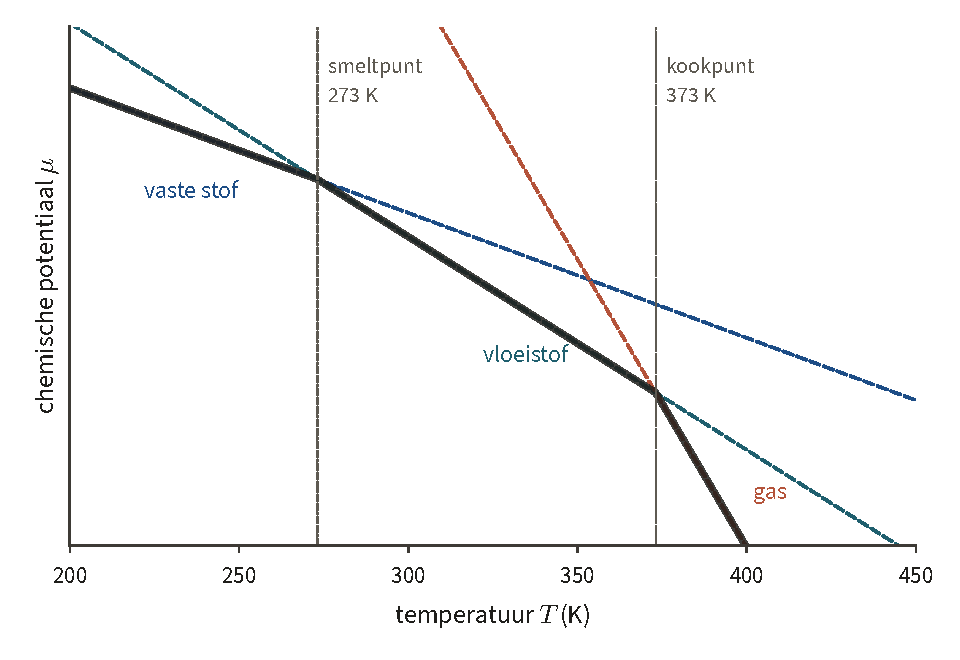
\includegraphics[width=0.7\linewidth]{Figuren/mu_temperatuur}
    \caption{Chemische potentiaal van vaste stof, vloeistof en gas van water bij \SI{1}{\bar} (schematisch op schaal, met $S_m$ = 41, 70 en \SI{189}{\joule\per\mole\per\kelvin}). De stabiele fase is telkens de laagste lijn (dik). De snijpunten zijn het smeltpunt en het kookpunt.}
    \label{fig:mu-T}
\end{figure}

Bij constante temperatuur stijgt $\mu$ met de druk, met helling $V_m$. Voor vloeistoffen en vaste stoffen is dat effect klein, voor gassen groot. Voor een ideaal gas ($V_m = RT/p$) geeft integratie vanaf de standaarddruk $p^\circ = \SI{1}{\bar}$:
\begin{equation}
\mu(T,p) = \mu^\circ(T) + RT \ln\frac{p}{p^\circ}.
\label{eq:mu-ideaalgas}
\end{equation}

\subsection{Fugaciteit: een veralgemening van de druk}
\label{sec:fugaciteit}
\label{sec:fugaciteitscoefficient}

Bij tientallen of honderden bar is een gas niet meer ideaal. Om de eenvoudige logaritmische vorm te behouden, vervangen we de druk door een effectieve druk, de \emph{fugaciteit} $f = \phi\,p$:
\begin{equation}
\mu = \mu^\circ + RT \ln\frac{f}{p^\circ} = \mu^\circ + RT \ln\frac{p}{p^\circ} + RT\ln\phi .
\end{equation}
De \emph{fugaciteitsco\"effici\"ent} $\phi$ meet de afwijking van ideaal gedrag ($\phi = 1$ voor een ideaal gas), net zoals de compressibiliteitsfactor $Z$ in hoofdstuk~\ref{ch:energie}. In de praktijk berekent men $\phi$ met een kubische toestandsvergelijking (Soave--Redlich--Kwong, Peng--Robinson).

\subsection{Activiteit: \'e\'en vorm voor elke fase}
\label{sec:activiteit}

In een ideaal gasmengsel draagt elke component bij met zijn partiële druk $p_i = y_ip$ (Dalton), zodat $\mu_i = \mu_i^\circ + RT\ln(p_i/p^\circ)$. Hetzelfde idee werkt voor elke fase.

\begin{definitie}{Chemische potentiaal via de activiteit}
Voor elke component $i$, in elke fase en bij elke samenstelling, geldt
\begin{equation}
\boxed{\mu_i = \mu_i^\circ + RT\ln a_i}
\label{eq:mu-activiteit}
\end{equation}
met $a_i$ de \emph{activiteit}: de dimensieloze ``effectieve concentratie'' die deze vergelijking exact maakt.
\end{definitie}

Voor een vloeistofmengsel schrijft men $a_i = \gamma_i x_i$, met $\gamma_i$ de \emph{activiteitsco\"effici\"ent}:
\begin{itemize}
\item $\gamma_i = 1$: ideaal gedrag, $a_i = x_i$ (voor een ideaal gas $a_i = p_i/p^\circ$);
\item $\gamma_i < 1$: de component voelt zich goed in het mengsel (sterkere aantrekking dan in zuivere toestand);
\item $\gamma_i > 1$: de component ``ontwijkt'' het mengsel;
\item een zuivere vloeistof of vaste stof in haar standaardtoestand heeft per afspraak $a_i = 1$.
\end{itemize}
Ethanol--water wijkt bijvoorbeeld zo sterk af van ideaal gedrag (waterstofbruggen) dat het een azeotroop vormt. Een kolomontwerp met $\gamma_i = 1$ zou daar volledig verkeerd uitkomen. Modellen voor $\gamma_i$ volgen in \S~\ref{sec:activiteitsmodellen}; in hoofdstuk~\ref{ch:reagerend} volstaan meestal $a_i \approx p_i/p^\circ$ en $a_i \approx 1$.

\subsection{Fase-evenwicht tussen twee fasen}
\label{sec:fase-evenwicht-voorwaarde}

Voor elke component geldt in evenwicht $\mu_i^{(\alpha)} = \mu_i^{(\beta)}$: tussen vast en vloeibaar, vloeistof en damp, twee vloeistoffen of twee kristalvormen. Bijna elk fase-evenwicht in de procestechnologie is een uitwerking van deze ene voorwaarde.


\subsection{De fasenregel van Gibbs}
\label{sec:fasenregel}

Hoeveel variabelen mag je vrij kiezen voor een systeem in evenwicht? Voor een zuivere stof die kookt, ligt de temperatuur vast zodra je de druk kiest: water kookt bij \SI{1}{atm} altijd bij \SI{100}{\celsius}. Voor een mengsel dat kookt, mag je ook nog de samenstelling kiezen. De \emph{fasenregel van Gibbs} telt dit precies:
\begin{equation}
\boxed{F = C - P + 2}
\label{eq:fasenregel}
\end{equation}
met $F$ het aantal \emph{vrijheidsgraden} (intensieve variabelen die je vrij kunt kiezen), $C$ het aantal componenten en $P$ het aantal fasen. De regel volgt uit een eenvoudige telling: elke fase heeft $T$, $p$ en $C-1$ onafhankelijke molfracties; elke component levert per extra fase \'e\'en evenwichtsvoorwaarde $\mu_i^{(\alpha)} = \mu_i^{(\beta)}$, en ook $T$ en $p$ zijn overal gelijk.
\begin{itemize}
\item Zuiver water, vloeistof + damp: $F = 1 - 2 + 2 = 1$. Kies $p$, dan ligt $T$ vast (de dampdruklijn).
\item Zuiver water op het tripelpunt: $F = 1 - 3 + 2 = 0$. Er is maar \'e\'en punt.
\item Benzeen--tolueen, vloeistof + damp: $F = 2 - 2 + 2 = 2$. Kies $p$ en $x$, dan liggen $T$ en $y$ vast. Dat is precies wat een VLE-diagram toont.
\end{itemize}

\section{Fase-evenwicht van zuivere stoffen: Clapeyron, Antoine en het fasediagram}

\subsection{De vergelijking van Clapeyron}
\label{sec:clapeyron}

Langs een evenwichtslijn blijven beide fasen in evenwicht, dus $\dd{\mu^{(\alpha)}} = \dd{\mu^{(\beta)}}$. Met $\dd{\mu} = V_m\,\dd{p} - S_m\,\dd{T}$ (vergelijking~\eqref{eq:dmu-fundamenteel}) voor elke fase en $\Delta S_{\text{trans}} = \Delta H_{\text{trans}}/T$ (hoofdstuk~\ref{ch:spontaniteit}) volgt de \emph{vergelijking van Clapeyron}:
\begin{equation}
\boxed{\;\frac{\dd{p}}{\dd{T}} = \frac{\Delta S_m}{\Delta V_m} = \frac{\Delta H_{\text{trans}}}{T\,\Delta V_m}\;}
\label{eq:clapeyron}
\end{equation}
Ze geldt voor elke faseovergang en geeft de helling van elke lijn in het fasediagram.

\begin{voorbeeld}{De smeltlijn van water}
IJs is minder dicht dan water, dus bij smelten is $\Delta V_m \approx \SI{-1.6e-6}{\metre\cubed\per\mole}$, met $\Delta H_{\text{fus}} = \SI{6.0}{\kilo\joule\per\mole}$:
\[
\frac{\dd{p}}{\dd{T}} = \frac{\SI{6000}{\joule\per\mole}}{(\SI{273.15}{\kelvin})(\SI{-1.6e-6}{\metre\cubed\per\mole})} \approx \SI{-140}{\bar\per\kelvin}.
\]
De helling is negatief: druk verlaagt het smeltpunt, maar je hebt \SI{140}{\bar} nodig voor \SI{1}{\kelvin}. Een schaatser haalt dat nauwelijks; de gladheid van ijs komt vooral van een dunne, vloeistofachtige oppervlaktelaag.
\end{voorbeeld}

\subsection{De vergelijking van Clausius--Clapeyron}
\label{sec:clausius-clapeyron}

Voor verdamping vereenvoudigt Clapeyron sterk: het dampvolume is veel groter dan het vloeistofvolume ($\Delta V_m \approx V_m^{(g)}$) en de damp is ongeveer ideaal ($V_m^{(g)} = RT/p$). Dan is $\dd{\ln p}/\dd{T} = \Delta H_{\text{vap}}/RT^2$, en met constante $\Delta H_{\text{vap}}$:
\begin{equation}
\boxed{\;\ln\frac{p_2}{p_1} = -\frac{\Delta H_{\text{vap}}}{R}\left(\frac{1}{T_2} - \frac{1}{T_1}\right)\;}
\label{eq:clausius-clapeyron-int}
\end{equation}
Een grafiek van $\ln p$ tegen $1/T$ is dus een rechte met helling $-\Delta H_{\text{vap}}/R$. Figuur~\ref{fig:dampdruk} toont hoe steil de dampdruk stijgt: elke \SI{20}{\kelvin} ongeveer een verdubbeling of meer.

\begin{figure}[htb]
    \centering
    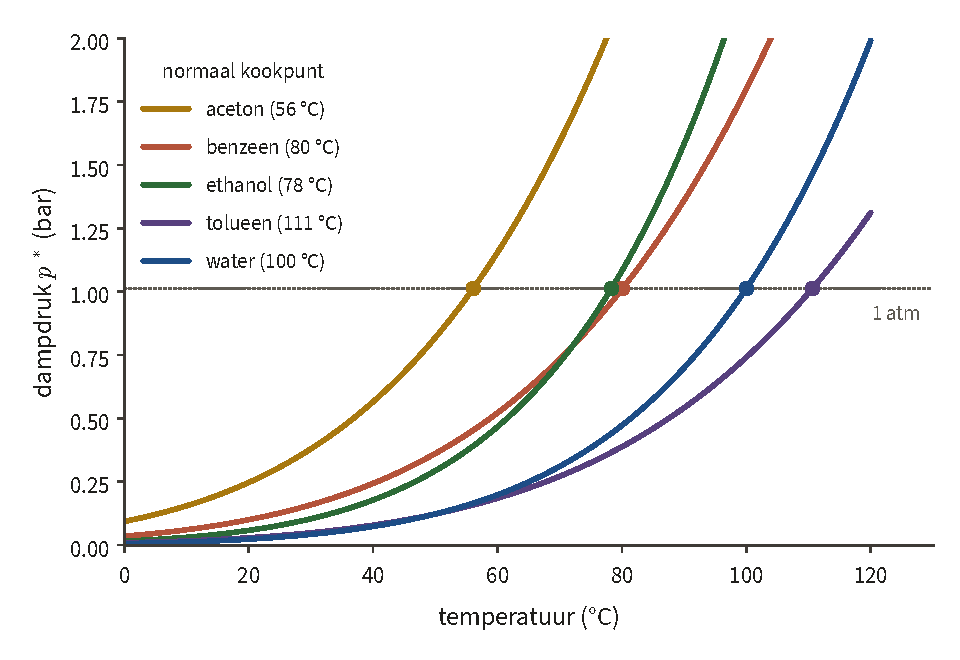
\includegraphics[width=0.7\linewidth]{Figuren/dampdruk}
    \caption{Dampdruk van vijf vloeistoffen. Waar een curve de lijn van \SI{1}{atm} snijdt, ligt het normale kookpunt. Benzeen en ethanol kruisen elkaar: bij kamertemperatuur is benzeen vluchtiger, boven ongeveer \SI{70}{\celsius} ethanol. Berekend met Antoine-constanten (bron: NIST WebBook; Dortmund Data Bank).}
    \label{fig:dampdruk}
\end{figure}

\begin{voorbeeld}{Dampdruk van water bij \SI{50}{\celsius}}
Uit het kookpunt ($p_1 = \SI{1.013}{\bar}$ bij \SI{373.15}{\kelvin}) en $\Delta H_{\text{vap}} = \SI{40.7}{\kilo\joule\per\mole}$:
\[
\ln\frac{p_2}{\SI{1.013}{\bar}} = -\frac{40700}{8.314}\left(\frac{1}{323.15} - \frac{1}{373.15}\right) = -3.42
\quad\Rightarrow\quad p_2 \approx \SI{36}{\milli\bar},
\]
dicht bij de gemeten \SI{35.6}{\milli\bar}.
\end{voorbeeld}

\subsection{De Antoine-vergelijking}
\label{sec:antoine}

Omdat $\Delta H_{\text{vap}}$ met de temperatuur verandert, gebruiken ingenieurs de empirische \emph{Antoine-vergelijking}:
\begin{equation}
\boxed{\;\log_{10} p^* = A - \frac{B}{T + C}\;}
\label{eq:antoine}
\end{equation}
De constanten $A$, $B$, $C$ staan in elke databank (NIST WebBook, Aspen Plus) en in de tabellenset.

\begin{voorbeeld}{Ethanol bij \SI{20}{\celsius}: controleer eerst de eenheden}
NIST geeft voor ethanol $A = 5.24677$, $B = 1598.673$, $C = -46.424$, met $p$ in bar en $T$ in kelvin. Andere bronnen gebruiken mmHg en \si{\celsius}, met totaal andere getallen. Controleer daarom eerst een bekend punt: bij $T = \SI{351.4}{\kelvin}$ geeft de formule \SI{1.013}{\bar}, het kookpunt van ethanol. Klopt. Dan bij \SI{293.15}{\kelvin}:
\[
\log_{10}p^* = 5.24677 - \frac{1598.673}{293.15 - 46.424} = -1.233
\quad\Rightarrow\quad p^* = \SI{58.5}{\milli\bar}
\]
(gemeten: \SI{59.5}{\milli\bar}).
\end{voorbeeld}

\subsection{Het fasediagram van een zuivere stof}
\label{sec:fasediagram}

De evenwichtslijnen samen vormen het \emph{fasediagram}: voor elke $(p, T)$ zie je welke fase stabiel is (figuur~\ref{fig:fasediagram}).

\begin{figure}[htb]
    \centering
    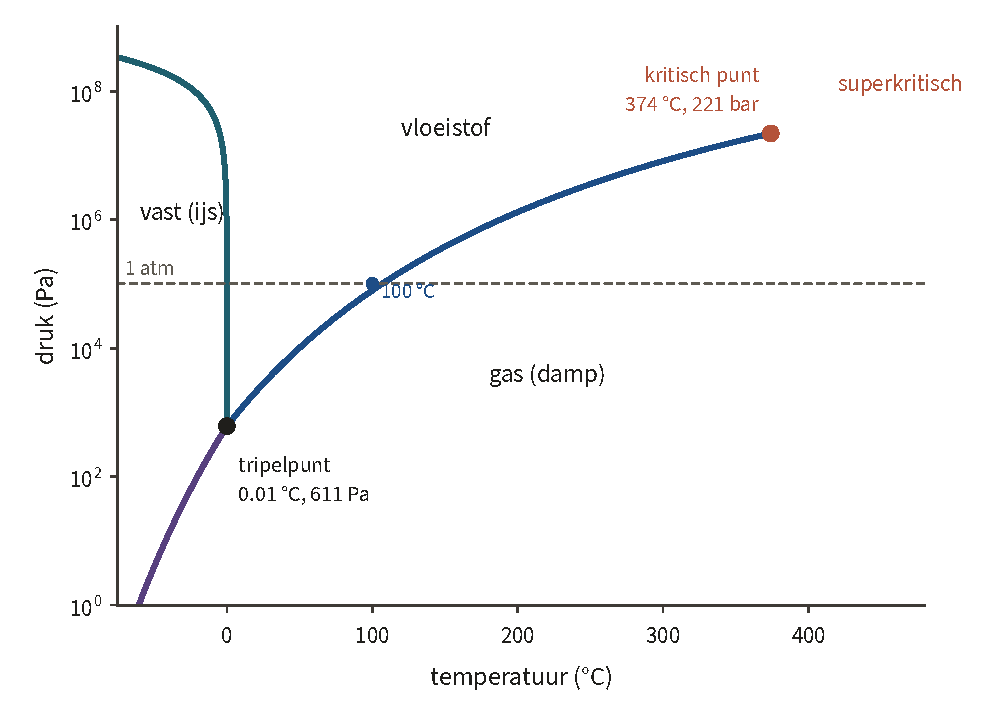
\includegraphics[width=0.7\linewidth]{Figuren/fasediagram}
    \caption{Fasediagram van water, met een logaritmische drukas. De dampdruklijn loopt van het tripelpunt tot het kritisch punt; de smeltlijn heeft een lichte \emph{negatieve} helling (hier overdreven getekend), zodat ijs bij hogere druk smelt. Bij \SI{1}{atm} kookt water bij \SI{100}{\celsius}.}
    \label{fig:fasediagram}
\end{figure}

\subsubsection{Het tripelpunt}
\label{sec:tripelpunt}

In het \emph{tripelpunt} bestaan drie fasen samen. Voor water: \SI{0.01}{\celsius} en \SI{611}{\pascal}. Onder die druk sublimeert ijs rechtstreeks: daarop berust vriesdrogen (koffie, vaccins).

\subsubsection{Het kritische punt}
\label{sec:kritisch-punt}

In het \emph{kritische punt} eindigt de dampdruklijn: vloeistof en damp worden ononderscheidbaar. Boven $T_c$ kan je een gas niet meer vloeibaar maken door samendrukken. Voor water: $T_c = \SI{374}{\celsius}$, $p_c = \SI{221}{\bar}$.

\subsubsection{Superkritische flu\"ida}
\label{sec:superkritisch}

Boven het kritische punt heeft een \emph{superkritisch flu\"idum} de dichtheid (en het oplosvermogen) van een vloeistof, maar diffundeert het als een gas. Superkritisch $\mathrm{CO_2}$ ($T_c = \SI{31}{\celsius}$, $p_c = \SI{74}{\bar}$) decaffe\"ineert koffie en extraheert hop, zonder resten van organisch solvent.

\section{Thermodynamica van mengsels en de wet van Raoult}

\subsection{Thermodynamica van mengsels}
\label{sec:thermodynamica-mengsels}

Ingenieurs werken bijna altijd met mengsels. In hoofdstuk~\ref{ch:spontaniteit} (\S~\ref{sec:waarschijnlijkheid-entropie}) zagen we dat mengen spontaan is door de toename van het aantal microtoestanden. Voor een \emph{ideaal} mengsel, waarin alle interacties even sterk zijn ($\Delta H_{\text{meng}} = 0$), geldt:
\begin{equation}
\Delta S_{\text{meng}} = -R \sum_i n_i \ln x_i > 0,
\qquad
\Delta G_{\text{meng}} = RT \sum_i n_i \ln x_i < 0.
\end{equation}

\begin{voorbeeld}{Minimale arbeid om lucht te scheiden}
Voor lucht ($x_{\mathrm{N_2}} = 0.79$, $x_{\mathrm{O_2}} = 0.21$) bij \SI{298}{\kelvin}:
\[
\Delta G_{\text{meng}} = RT(0.79\ln 0.79 + 0.21\ln 0.21) = \SI{-1.17}{\kilo\joule\per\mole}.
\]
Scheiden kost dus minstens \SI{1.17}{\kilo\joule} per mol lucht. Een cryogene luchtscheider haalt een rendement van 15 tot \SI{25}{\percent} van dat minimum.
\end{voorbeeld}

\subsubsection{Niet-ideale mengsels}
\label{sec:niet-ideale-mengsels}

Zijn de A--B-interacties zwakker dan de A--A- en B--B-interacties, dan is $\Delta H_{\text{meng}} > 0$ (hoofdstuk~\ref{ch:intermoleculair}, \S~\ref{sec:hildebrand}). In $\Delta G_{\text{meng}} = \Delta H_{\text{meng}} - T\Delta S_{\text{meng}}$ wordt het entropievoordeel dan deels of helemaal tenietgedaan. Figuur~\ref{fig:mengen-G} toont wat er gebeurt: bij een sterk endotherme menging krijgt de curve twee minima. Een mengsel tussen die minima valt spontaan uiteen in twee fasen (water en olie, \S~\ref{sec:lle}).

\begin{figure}[htb]
    \centering
    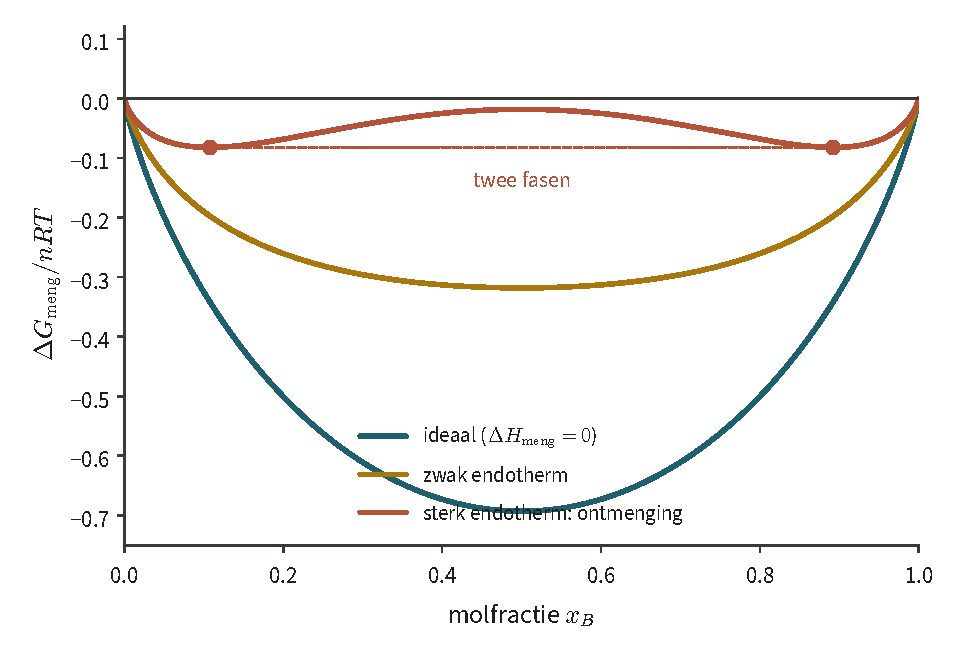
\includegraphics[width=0.7\linewidth]{Figuren/mengen_G}
    \caption{Gibbs-energie van mengen voor een binair mengsel met $\Delta H_{\text{meng}} = \chi RT\,x_A x_B$ (regelmatige oplossing). Voor $\chi > 2$ ontstaan twee minima: mengsels tussen de twee punten op de gemeenschappelijke raaklijn splitsen in twee vloeistoffasen.}
    \label{fig:mengen-G}
\end{figure}

\subsection{De chemische potentiaal in een mengsel}
\label{sec:mu-mengsel}

Afleiden van $G = \sum_i n_i \mu_i^* + RT \sum_i n_i \ln x_i$ naar $n_i$ geeft de chemische potentiaal in een ideaal mengsel:
\begin{equation}
\boxed{\;\mu_i = \mu_i^* + RT \ln x_i\;}
\label{eq:mu-mengsel-ideaal}
\end{equation}
Verdunnen verlaagt $\mu_i$: een component in een mengsel ``ontsnapt'' minder graag dan als zuivere stof.

\subsection{De wet van Raoult}
\label{sec:raoult}

Stel $\mu_i$ in de vloeistof (vergelijking~\eqref{eq:mu-mengsel-ideaal}) gelijk aan $\mu_i$ in de ideale damp, en je vindt de \emph{wet van Raoult}:
\begin{equation}
\boxed{\;p_i = x_i\,p_i^*\;}
\label{eq:raoult}
\end{equation}
De parti\"ele dampdruk is evenredig met de molfractie in de vloeistof; $p_i^*$ volgt uit Antoine. Voor een binair mengsel geeft Dalton de \emph{bubbelpuntsdruk} en de dampsamenstelling:
\begin{equation}
P = x_A p_A^* + x_B p_B^*, \qquad y_i = \frac{x_i p_i^*}{P}.
\end{equation}

\begin{voorbeeld}{Benzeen--tolueen bij \SI{90}{\celsius}}
Met $x_A = 0.40$ benzeen, $p_A^* = \SI{1.35}{\bar}$ en $p_B^* = \SI{0.54}{\bar}$:
\[
P = 0.40 \cdot 1.35 + 0.60 \cdot 0.54 = \SI{0.864}{\bar}, \qquad y_A = \frac{0.40 \cdot 1.35}{0.864} = 0.625.
\]
De damp bevat \SI{62.5}{\percent} benzeen, de vloeistof maar \SI{40}{\percent}. Dat verschil is de basis van destillatie.
\end{voorbeeld}

\subsection{Relatieve vluchtigheid}
\label{sec:relatieve-vluchtigheid}

Hoe makkelijk twee componenten door destillatie te scheiden zijn, vat de \emph{relatieve vluchtigheid} samen:
\begin{equation}
\boxed{\;\alpha_{AB} = \frac{y_A/x_A}{y_B/x_B} = \frac{p_A^*}{p_B^*}\;}
\end{equation}
(de tweede gelijkheid voor ideale mengsels). Bij $\alpha \approx 1$ is destillatie praktisch onmogelijk, bij $\alpha \approx 2$ eenvoudig, en bij $\alpha \geq 5$ zeer eenvoudig. Voor benzeen--tolueen bij \SI{90}{\celsius} is $\alpha = 1.35/0.54 = 2.5$: een klassiek, goed scheidbaar mengsel.

\section{Het damp-vloeistofdiagram: hefboomwet en azeotropen}

\subsection{Zelf een VLE-diagram opstellen}
\label{sec:vle-diagram}

Een damp-vloeistofdiagram (VLE-diagram) toont voor een binair mengsel welke vloeistof met welke damp in evenwicht is. Voor een ideaal mengsel kun je het volledig zelf opstellen met twee ingredi\"enten: de wet van Raoult en de dampdrukken van de zuivere componenten (Antoine, \S~\ref{sec:antoine}). Er zijn drie gangbare voorstellingen.

\subsubsection{Het $P$--$x$--$y$-diagram (constante temperatuur)}

Kies de temperatuur, bereken $p_A^*$ en $p_B^*$, en doorloop $x_A$ van 0 tot 1:
\begin{enumerate}
\item bubbelpuntdruk: $P = x_A p_A^* + (1 - x_A) p_B^*$;
\item dampsamenstelling: $y_A = x_A p_A^*/P$;
\item zet $P$ uit tegen $x_A$ (de \emph{bubbelpuntlijn}, een rechte) en tegen $y_A$ (de \emph{dauwpuntlijn}, gekromd).
\end{enumerate}
Boven de bubbelpuntlijn is het mengsel volledig vloeibaar, onder de dauwpuntlijn volledig damp. Daartussen liggen vloeistof en damp naast elkaar (figuur~\ref{fig:vle-diagram}). Een horizontale lijn in dat gebied verbindt een vloeistof met de damp waarmee ze in evenwicht is: een \emph{bindlijn}.

\begin{figure}[htb]
    \centering
    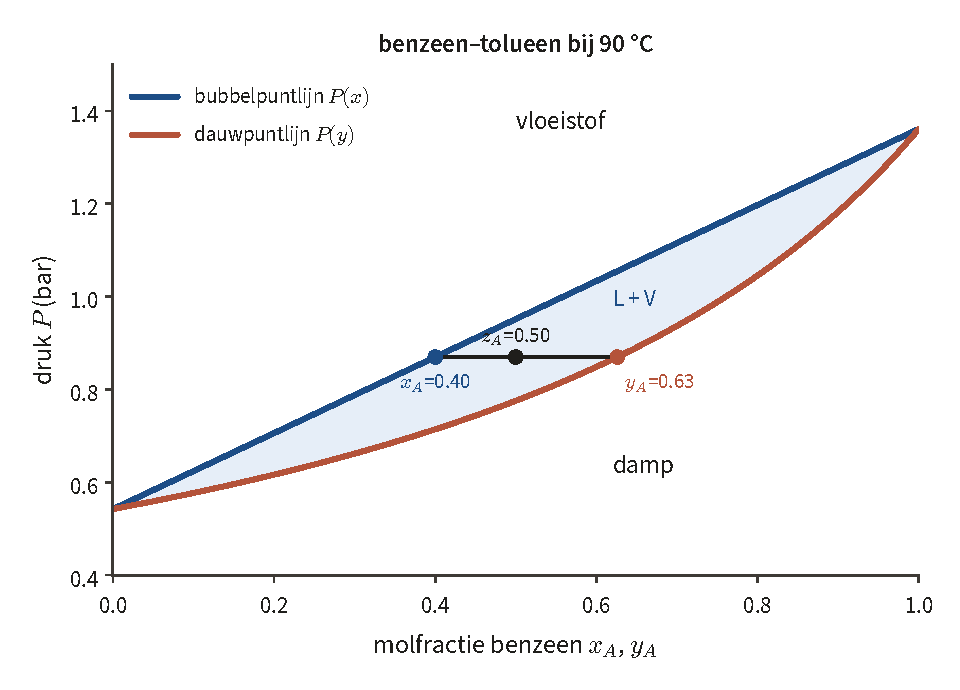
\includegraphics[width=0.75\linewidth]{Figuren/pxy_benzeen_tolueen}
    \caption{$P$--$x$--$y$-diagram van benzeen (A) en tolueen (B) bij \SI{90}{\celsius}, berekend met de wet van Raoult en de Antoinevergelijking. De bindlijn bij $P \approx \SI{0.87}{\bar}$ verbindt vloeistof met $x_A = 0.40$ en damp met $y_A = 0.63$; het punt $z_A = 0.50$ hoort bij het voorbeeld van de hefboomwet (\S~\ref{sec:hefboomwet}).}
    \label{fig:vle-diagram}
\end{figure}

\subsubsection{Het $T$--$x$--$y$-diagram (constante druk)}

In een destillatiekolom ligt de druk vast en varieert de temperatuur. Het $T$--$x$--$y$-diagram is daarom het meest gebruikte. Het opstellen vraagt \'e\'en extra stap, omdat $p^*$ afhangt van de onbekende temperatuur:
\begin{enumerate}
\item kies $x_A$;
\item zoek de temperatuur waarbij $x_A p_A^*(T) + (1 - x_A) p_B^*(T) = P$. Dat is een vergelijking in \'e\'en onbekende, op te lossen met \emph{Doelzoeken} in Excel of door een paar temperaturen te proberen;
\item bereken $y_A = x_A p_A^*(T)/P$;
\item herhaal voor andere $x_A$ en zet $T$ uit tegen $x_A$ en $y_A$.
\end{enumerate}
De bubbelpuntlijn ligt nu \emph{onder}: een vloeistof begint te koken wanneer je ze opwarmt tot op die lijn. De dauwpuntlijn ligt erboven (figuur~\ref{fig:txy}).

\begin{voorbeeld}{Kookpunt van een benzeen--tolueenmengsel bij 1 atm}
Gevraagd: de kooktemperatuur en de eerste damp van een vloeistof met $x_A = 0.40$ bij $P = \SI{1.013}{\bar}$. Antoine (\si{mmHg}, \si{\celsius}): benzeen $A = 6.90565$, $B = 1211.033$, $C = 220.790$; tolueen $A = 6.95464$, $B = 1344.800$, $C = 219.482$.

Probeer \SI{95}{\celsius}: $p_A^* = \SI{1.569}{\bar}$, $p_B^* = \SI{0.636}{\bar}$, en $0.40(1.569) + 0.60(0.636) = \SI{1.009}{\bar}$: net te laag. Bij \SI{95.1}{\celsius} klopt de som. Daar is $y_A = 0.40 \times 1.575/1.013 = 0.62$.

De eerste damp bevat dus 62\,\% benzeen, tegenover 40\,\% in de vloeistof. Condenseer je die damp en laat je hem opnieuw koken, dan wordt hij nog rijker. Dat is het principe van een destillatiekolom: elke schotel is een nieuwe stap tussen de bubbelpunt- en de dauwpuntlijn.
\end{voorbeeld}

\subsubsection{Het $x$--$y$-diagram}

Zet je voor elk punt $y_A$ uit tegen $x_A$, dan krijg je de \emph{evenwichtslijn} van het $x$--$y$-diagram (figuur~\ref{fig:txy}, rechts). Hoe verder die lijn boven de diagonaal $y = x$ ligt, hoe gemakkelijker de scheiding. Voor een ideaal mengsel met constante relatieve vluchtigheid $\alpha$ geldt
\begin{equation}
y_A = \frac{\alpha\,x_A}{1 + (\alpha - 1)\,x_A}.
\label{eq:xy-alpha}
\end{equation}
Dit diagram is het vertrekpunt van de grafische methode van McCabe--Thiele, waarmee je in de cursus Scheidingstechnologie het aantal schotels van een destillatiekolom bepaalt.

\begin{figure}[htb]
    \centering
    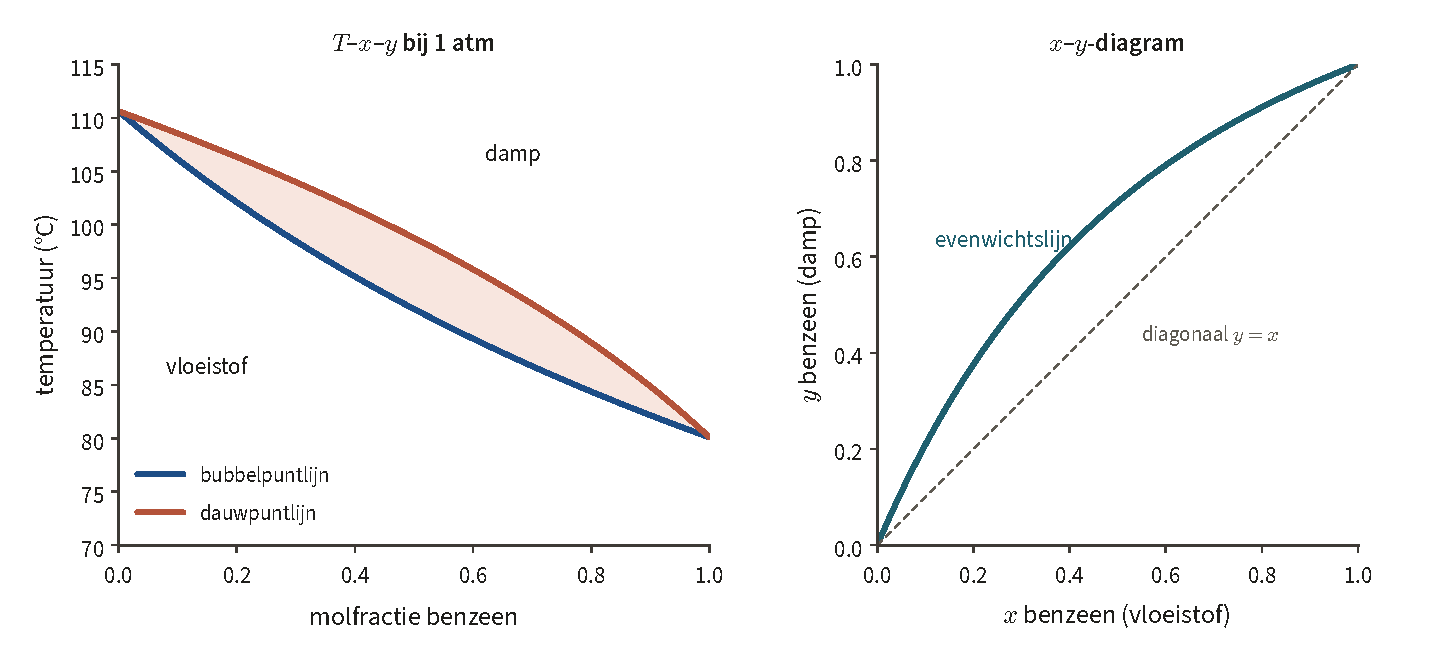
\includegraphics[width=\linewidth]{Figuren/txy_benzeen_tolueen}
    \caption{Links: $T$--$x$--$y$-diagram van benzeen--tolueen bij \SI{1}{atm}. Rechts: het bijbehorende $x$--$y$-diagram. Beide berekend met Raoult en Antoine; zuiver benzeen kookt bij \SI{80.1}{\celsius}, zuiver tolueen bij \SI{110.6}{\celsius}.}
    \label{fig:txy}
\end{figure}

\subsection{De hefboomwet (lever rule)}
\label{sec:hefboomwet}

Wanneer een mengsel zich in het tweefasengebied bevindt, geldt een massabalans die de verhouding van vloeistof en damp vastlegt. Beschouw een totaal aantal mol $n_{\text{tot}}$ met globale molfractie $z_A$, dat splitst in een vloeistoffase ($n_L$, molfractie $x_A$) en een dampfase ($n_V$, molfractie $y_A$). De massabalans voor component $A$ luidt:
\[
n_{\text{tot}} z_A = n_L x_A + n_V y_A.
\]
Met $n_{\text{tot}} = n_L + n_V$ volgt na herschikking de \emph{hefboomwet}:
\begin{equation}
\boxed{\;\frac{n_L}{n_V} = \frac{y_A - z_A}{z_A - x_A}\;}
\label{eq:hefboomwet}
\end{equation}
De verhouding van vloeistof- en damphasen wordt dus bepaald door de afstand van het globale punt tot de bubbelpunt- en dauwpuntcurve, analoog aan een hefboom rond een steunpunt.

\begin{voorbeeld}{Toepassing van de hefboomwet}
Voor het benzeen--tolueenmengsel bij \SI{90}{\celsius} en $P = \SI{0.864}{\bar}$ geldt $x_A = 0.40$ en $y_A = 0.625$ (uit het eerdere voorbeeld). Een globale samenstelling $z_A = 0.50$ geeft:
\[
\frac{n_L}{n_V} = \frac{0.625 - 0.50}{0.50 - 0.40} = \frac{0.125}{0.10} = 1.25.
\]
Van elke mol mengsel bevindt zich dus $n_L = 0.56$ mol in de vloeistoffase en $n_V = 0.44$ mol in de dampfase. Deze eenvoudige berekening vormt het vertrekpunt van het ontwerp van een destillatiekolom.
\end{voorbeeld}

\subsection{Azeotropen}
\label{sec:azeotropen}

Re\"ele mengsels wijken af van Raoult. Is de afwijking groot genoeg, dan krijgt de $P$--$x$-curve een maximum of minimum. Daar zijn vloeistof en damp even samengesteld: een \emph{azeotroop} (figuur~\ref{fig:azeotroop}). Destillatie raakt daar niet voorbij.

\begin{figure}[htb]
    \centering
    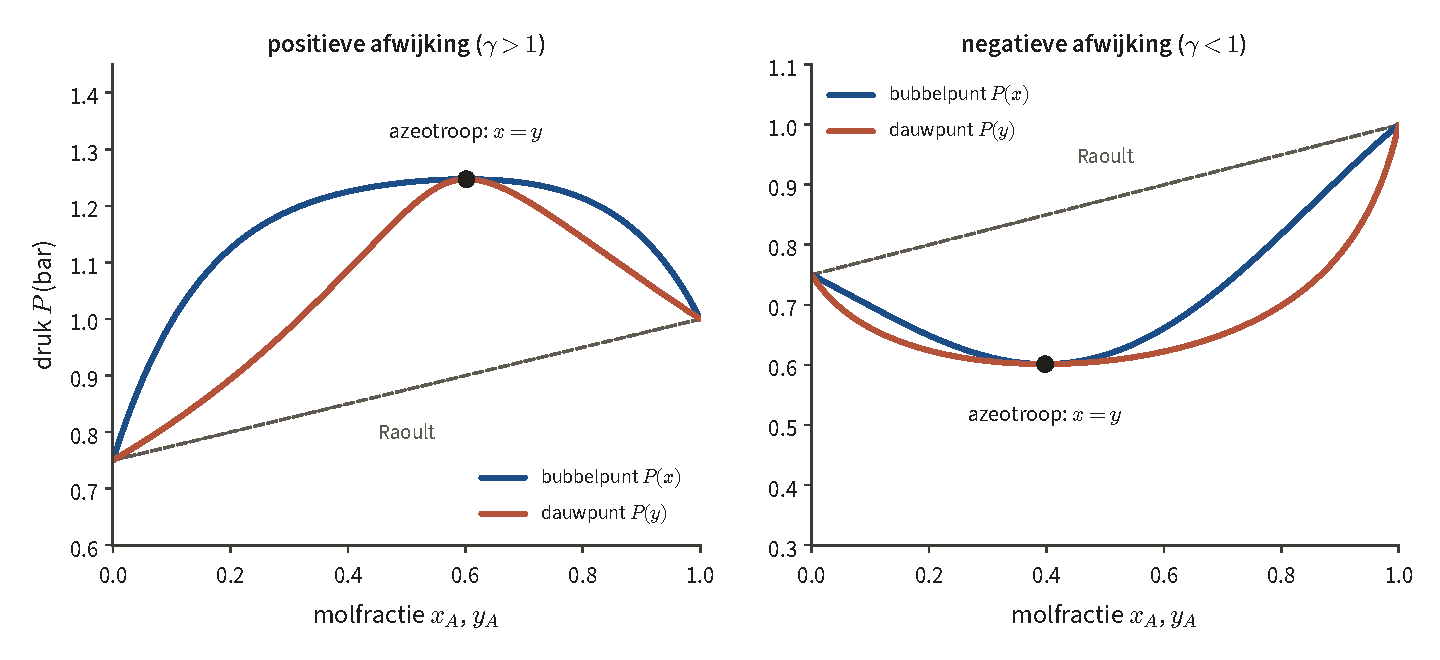
\includegraphics[width=\linewidth]{Figuren/azeotroop}
    \caption{$P$--$x$--$y$-diagrammen bij constante temperatuur voor een mengsel met positieve (links) en negatieve (rechts) afwijking van Raoult (Margules, $A = \pm 1.4$). In het extremum raken bubbelpunt- en dauwpuntlijn elkaar: de azeotroop. De stippellijn is de wet van Raoult.}
    \label{fig:azeotroop}
\end{figure}

\begin{itemize}
\item \textbf{Positieve afwijking} (A--B-interacties zwakker): dampdruk boven Raoult, dus een \emph{minimaal kokende} azeotroop. Ethanol--water kookt bij \SI{78.2}{\celsius} en $x_{\text{eth}} = 0.894$ (\SI{95.6}{\percent} in massa), net onder zuiver ethanol (\SI{78.4}{\celsius}). Daarom haal je met gewone destillatie geen zuiverdere ethanol.
\item \textbf{Negatieve afwijking} (A--B-interacties sterker): dampdruk onder Raoult, dus een \emph{maximaal kokende} azeotroop. Aceton--chloroform kookt bij \SI{64.5}{\celsius}, boven beide zuivere stoffen, door een waterstofbrug tussen \ce{C=O} en \ce{Cl3C-H} (hoofdstuk~\ref{ch:intermoleculair}, \S~\ref{sec:waterstofbruggen}). Zoutzuur--water kookt constant bij \SI{110}{\celsius} en \SI{20}{\percent} HCl.
\end{itemize}

\section{Re\"ele mengsels: activiteit en activiteitsco\"effici\"entmodellen}

\subsection{Re\"ele mengsels en activiteit}
\label{sec:activiteit-mengsel}

Voor re\"ele mengsels vervangen we de molfractie door de activiteit (\S~\ref{sec:activiteit}), met de \emph{activiteitsco\"effici\"ent} $\gamma_i$ als correctiefactor:
\begin{equation}
\mu_i = \mu_i^* + RT \ln a_i, \qquad
\boxed{\;a_i = \gamma_i\,x_i\;}
\label{eq:activiteit-mengsel}
\end{equation}
Raoult wordt dan $p_i = \gamma_i x_i p_i^*$ (gemodificeerde Raoult). Bij $\gamma_i > 1$ ontsnapt de component makkelijker dan ideaal (positieve afwijking), bij $\gamma_i < 1$ wordt hij beter vastgehouden (negatieve afwijking). Voor de zuivere stof ($x_i \to 1$) gaat $\gamma_i$ altijd naar 1.

\subsubsection{De wet van Henry}
\label{sec:henry}

Een sterk verdunde component is volledig omringd door oplosmiddel. Zijn ``ontsnappingsneiging'' hangt dan af van de interactie met dat oplosmiddel, niet met zijn eigen soort, en $\gamma_i$ wordt constant ($\gamma_i^\infty$). Dat geeft de \emph{wet van Henry}:
\begin{equation}
\boxed{\;p_i = x_i\,H_i\;}
\label{eq:henry}
\end{equation}
met $H_i = \gamma_i^\infty p_i^*$ een eigenschap van het paar opgeloste stof--oplosmiddel. In dezelfde oplossing volgt het oplosmiddel dus Raoult en de opgeloste stof Henry (figuur~\ref{fig:raoult-henry}). Henry beschrijft vooral de oplosbaarheid van gassen ($\mathrm{O_2}$, $\mathrm{CO_2}$, $\mathrm{N_2}$) in water.

\begin{figure}[htb]
    \centering
    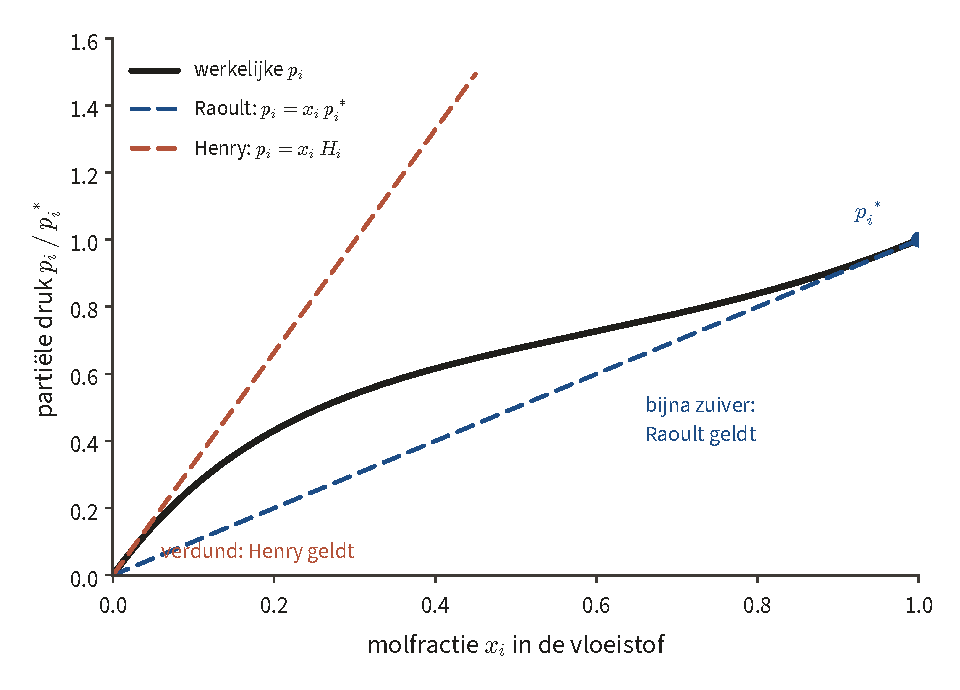
\includegraphics[width=0.7\linewidth]{Figuren/raoult_henry}
    \caption{Parti\"ele dampdruk van een component met positieve afwijking van Raoult. Bij hoge molfractie (bijna zuiver) volgt de curve de wet van Raoult; in sterke verdunning volgt ze de wet van Henry, met een andere helling $H_i$. Daartussen is een activiteitsco\"effici\"entmodel nodig.}
    \label{fig:raoult-henry}
\end{figure}

\begin{voorbeeld}{Waarom een fles spuitwater bruist}
Voor $\mathrm{CO_2}$ in water bij \SI{25}{\celsius} is $H \approx \SI{1640}{\bar}$. Onder \SI{3}{\bar} $\mathrm{CO_2}$ in de fles is $x_{\mathrm{CO_2}} = 3/1640 = 1.8\times10^{-3}$. Na openen is $p_{\mathrm{CO_2}} \approx \SI{4e-4}{\bar}$ en zakt het evenwicht naar $2.4\times10^{-7}$: \num{7500} keer minder. Het overtollige gas komt vrij als bellen.
\end{voorbeeld}

\paragraph{Let op de eenheden.}
Tabellen geven vaak de oplosbaarheid $k_\mathrm{H} = c_i/p_i$ in \si{\mole\per\litre\per\bar}. Voor verdunde waterige oplossingen (\SI{55.5}{\mole} water per liter) is $H_i\,(\si{\bar}) \approx 55.5/k_\mathrm{H}$. Een verwisseling geeft al snel een factor $10^4$ fout.

\paragraph{Temperatuur.}
Gassen lossen bijna altijd \emph{slechter} op bij hogere temperatuur: oplossen is exotherm (Le Chatelier). Zoals bij Clausius--Clapeyron is $\ln k_\mathrm{H}$ ongeveer lineair in $1/T$.

\begin{toepassing}{Zuurstof in water: van vissenkom tot stoomketel}
Voor zuurstof in water bij \SI{25}{\celsius} is $k_\mathrm{H} = \SI{1.3e-3}{\mole\per\litre\per\bar}$. Met \SI{0.21}{\bar} zuurstof in lucht geeft dat $c_{\ce{O2}} = \SI{2.7e-4}{\mole\per\litre} \approx \SI{8.7}{\milli\gram\per\litre}$. Bij \SI{5}{\celsius} is dat ongeveer \SI{13}{\milli\gram\per\litre}, bij \SI{35}{\celsius} nog \SI{7.3}{\milli\gram\per\litre}. Vissen hebben minstens \SIrange{4}{5}{\milli\gram\per\litre} nodig: in een warme zomernacht wordt het kritiek, en waterzuiveringen blazen daarom lucht in.

Een stoomketel wil net \emph{geen} zuurstof, omdat die het staal corrodeert (hoofdstuk~\ref{ch:elektrochemie}). In een \emph{ontgasser} wordt het voedingswater met stoom tot het kookpunt verwarmd; de stoom voert de vrijgekomen zuurstof af tot onder \SI{10}{\micro\gram\per\litre}.
\end{toepassing}

\subsection{Modellen voor activiteitsco\"effici\"enten}
\label{sec:activiteitsmodellen}

Om $\gamma_i$ te berekenen gebruikt men modellen met enkele parameters, gefit op metingen. Het eenvoudigste is \emph{Margules met \'e\'en parameter}:
\begin{equation}
\ln \gamma_A = A\, x_B^2, \qquad \ln \gamma_B = A\, x_A^2.
\end{equation}
$A > 0$ geeft positieve en $A < 0$ negatieve afwijking; bij oneindige verdunning is $\gamma^\infty = e^A$ (figuur~\ref{fig:margules}). Voor aceton--chloroform bij \SI{35}{\celsius} is $A = -0.84$, zodat bij $x = 0.5$: $\gamma = e^{-0.21} = 0.81$.

\begin{figure}[htb]
    \centering
    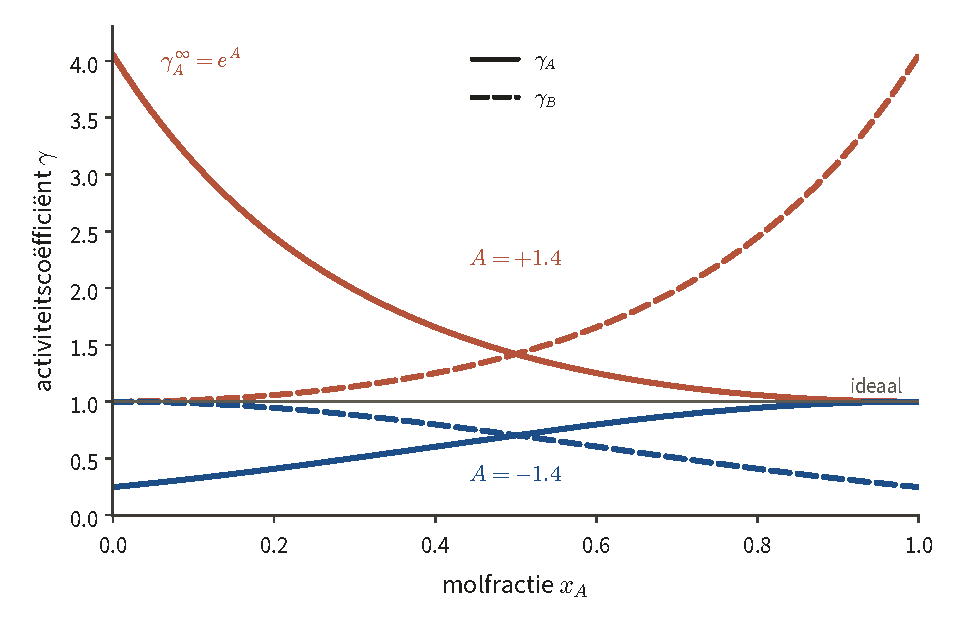
\includegraphics[width=0.7\linewidth]{Figuren/margules}
    \caption{Activiteitsco\"effici\"enten volgens Margules (\'e\'en parameter). Elke component nadert $\gamma = 1$ als hij bijna zuiver is, en wijkt het sterkst af bij oneindige verdunning. Deze $\gamma$'s leveren de azeotropen van figuur~\ref{fig:azeotroop}.}
    \label{fig:margules}
\end{figure}

Re\"ele mengsels zijn vaak asymmetrisch. Daarvoor bestaan modellen met twee of drie parameters (tabel~\ref{tab:gamma-modellen}). Je hoeft hun formules niet te kennen: processimulators zoals Aspen Plus bevatten ze, samen met parameters uit databanken. Belangrijk is wel te weten wat elk model kan.

\begin{table}[htb]
\centering
\small
\begin{tabular}{lcl}
\toprule
Model & Parameters & Geschikt voor \\
\midrule
Margules (1 of 2) & 1--2 & snelle schatting, onderwijs \\
Van Laar & 2 & eenvoudige niet-ideale mengsels \\
Wilson & 2 & volledig mengbare mengsels; \emph{geen} LLE \\
NRTL & 3 & algemeen: VLE \'en LLE \\
UNIQUAC & 2 & zoals NRTL, houdt rekening met molecuulgrootte \\
\bottomrule
\end{tabular}
\caption{Activiteitsco\"effici\"entmodellen voor vloeistofmengsels. In de procesindustrie zijn Wilson en NRTL het meest gebruikt.}
\label{tab:gamma-modellen}
\end{table}

\section{Vloeistof-vloeistof- en vast-vloeistofevenwicht}

\subsection{Vloeistof-vloeistofevenwicht (LLE)}
\label{sec:lle}

Is $\Delta H_{\text{meng}}$ sterk positief (zeer verschillende Hildebrand-parameters, hoofdstuk~\ref{ch:intermoleculair}), dan krijgt $\Delta G_{\text{meng}}$ twee minima en splitst het mengsel in twee vloeistoffasen (figuur~\ref{fig:mengen-G}): water--olie, water--fenol, polymeer--oplosmiddel. Dat \emph{vloeistof-vloeistofevenwicht} is de basis van extractie, nuttig voor componenten die moeilijk te destilleren zijn.

\subsubsection{De Nernst-verdelingswet}
\label{sec:nernst}

Een component die verdeeld raakt over twee onmengbare fasen heeft in beide dezelfde $\mu$. In verdunde oplossing geeft dat een constante verhouding, de \emph{verdelingswet van Nernst}:
\begin{equation}
\boxed{\;K_D = \frac{c_i^{(\alpha)}}{c_i^{(\beta)}}\;}
\label{eq:nernst-verdeling}
\end{equation}

\begin{voorbeeld}{Extractie van jodium}
Jodium verdeelt zich tussen $\mathrm{CCl_4}$ en water met $K_D \approx 86$. Extraheer je \SI{1}{\litre} waterige oplossing (\SI{0.1}{\mole\per\litre}) met \SI{0.5}{\litre} $\mathrm{CCl_4}$, dan blijft in het water
\[
c_{\text{water}} = 0.1 \cdot \frac{V_w}{V_w + K_D V_o} = 0.1 \cdot \frac{1}{1 + 86 \cdot 0.5} = \SI{0.0023}{\mole\per\litre}.
\]
E\'en stap verwijdert dus \SI{97.7}{\percent} van het jodium.
\end{voorbeeld}

\subsubsection{Ternaire diagrammen}
\label{sec:ternair}

Bij vloeistof-vloeistofextractie zijn er minstens drie componenten: de \emph{drager} (bv.\ water), de \emph{opgeloste stof} die je wilt winnen (bv.\ aceton) en het \emph{extractiemiddel} (bv.\ methylisobutylketon, MIBK). Hun evenwicht stel je voor in een \emph{ternair diagram}: een gelijkzijdige driehoek (figuur~\ref{fig:ternair}).
\begin{itemize}
\item Elke hoek is een zuivere component; elke zijde een binair mengsel.
\item Een punt binnen de driehoek is een mengsel van alle drie. De massafractie van een component lees je af als de afstand tot de zijde tegenover zijn hoek: op die zijde is ze 0, in de hoek 1. De drie fracties tellen altijd op tot 1.
\item De \emph{binodale curve} begrenst het gebied waarin het mengsel in twee vloeistoffasen uiteenvalt. Binnen dat gebied verbinden \emph{bindlijnen} de twee fasen die met elkaar in evenwicht zijn: het \emph{raffinaat} (waterrijk, links) en het \emph{extract} (MIBK-rijk, rechts).
\item Waar de bindlijnen krimpen tot een punt, worden beide fasen identiek: het \emph{plooipunt}.
\end{itemize}

Het belangrijkste rekeninstrument is opnieuw de hefboomwet. Meng je twee stromen F en S, dan ligt het mengpunt M op de rechte FS, en de verhouding van de hoeveelheden is omgekeerd evenredig met de afstanden: $m_\mathrm{F}/m_\mathrm{S} = \overline{\mathrm{MS}}/\overline{\mathrm{MF}}$. Valt M in het tweefasengebied, dan splitst het mengsel langs de bindlijn door M in raffinaat R en extract E.

\begin{figure}[htb]
    \centering
    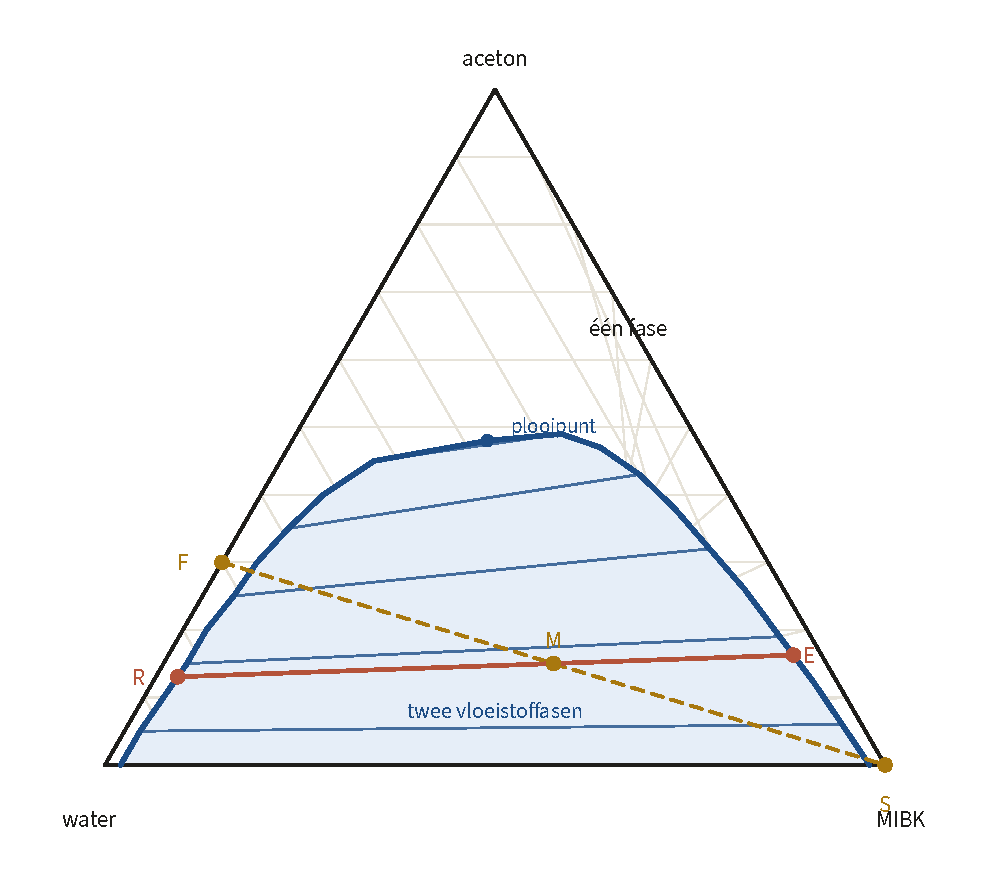
\includegraphics[width=0.72\linewidth]{Figuren/ternair}
    \caption{Ternair diagram water--aceton--MIBK bij \SI{25}{\celsius} (massafracties, benaderende waarden). Binnen de binodale curve vormen zich twee vloeistoffasen, verbonden door bindlijnen. Het voorbeeld: voeding F (30\,\% aceton in water) wordt gemengd met evenveel zuiver MIBK (S) tot M, dat splitst in raffinaat R en extract E.}
    \label{fig:ternair}
\end{figure}

\begin{voorbeeld}{Aceton uit water extraheren met MIBK}
\SI{100}{\kilo\gram} water met \SI{30}{\percent} aceton wordt gemengd met \SI{100}{\kilo\gram} zuiver MIBK.

\textbf{Mengpunt.} Het mengsel van \SI{200}{\kilo\gram} bevat 30 kg aceton, 70 kg water en 100 kg MIBK: M = (15\,\% aceton, 35\,\% water, 50\,\% MIBK). Dat ligt in het midden van de rechte FS, en binnen de binodale curve.

\textbf{Bindlijn.} De bindlijn door M (figuur~\ref{fig:ternair}) geeft het raffinaat R = (13\,\% aceton, 84\,\% water, 3\,\% MIBK) en het extract E = (16\,\% aceton, 4\,\% water, 80\,\% MIBK).

\textbf{Hefboomwet.} Met een acetonbalans: $200 \times 0.15 = 0.130\,m_\mathrm{R} + 0.163\,m_\mathrm{E}$ en $m_\mathrm{R} + m_\mathrm{E} = 200$, dus $m_\mathrm{E} = \SI{121}{\kilo\gram}$ en $m_\mathrm{R} = \SI{79}{\kilo\gram}$.

Het extract bevat $121 \times 0.163 = \SI{19.7}{\kilo\gram}$ aceton: twee derde van de aceton is in \'e\'en stap overgegaan naar het MIBK. Het raffinaat bevat nog \SI{10}{\kilo\gram} aceton. Met een tweede extractiestap op het raffinaat, of een tegenstroomkolom, haal je bijna alles. Hoeveel stappen nodig zijn, leer je in de cursus Scheidingstechnologie.
\end{voorbeeld}

\subsection{Vast-vloeistofevenwicht (SLE)}
\label{sec:sle}

Het evenwicht tussen een vaste stof en een vloeistof speelt een centrale rol bij kristallisatie, legeringen en zuiveringsprocessen. Net als bij VLE wordt het SLE bepaald door de gelijkheid van de chemische potentialen, maar de rol van beide fasen is gewijzigd.

\subsubsection{Eutectische diagrammen}
\label{sec:eutecticum}

Voor een binair systeem $A$--$B$ met beperkte vaste-mengbaarheid vertoont het fasediagram een \emph{eutecticum}. Het \emph{eutectisch punt} is de combinatie van samenstelling en temperatuur waarbij vloeistof, vaste stof $A$ en vaste stof $B$ (of twee vaste oplossingen) gelijktijdig co\"existeren. Bij afkoelen van een vloeistof met eutectische samenstelling stollen beide componenten simultaan bij een vaste temperatuur, analoog aan een zuivere stof.

Voor mengsels met een andere samenstelling begint de stolling bij een hogere temperatuur, waarbij eerst de ene component als vaste fase uitkristalliseert. De resterende vloeistof verandert in samenstelling langs de \emph{liquidus}-curve naarmate de temperatuur daalt, tot het eutectisch punt wordt bereikt.

\begin{figure}[htb]
    \centering
    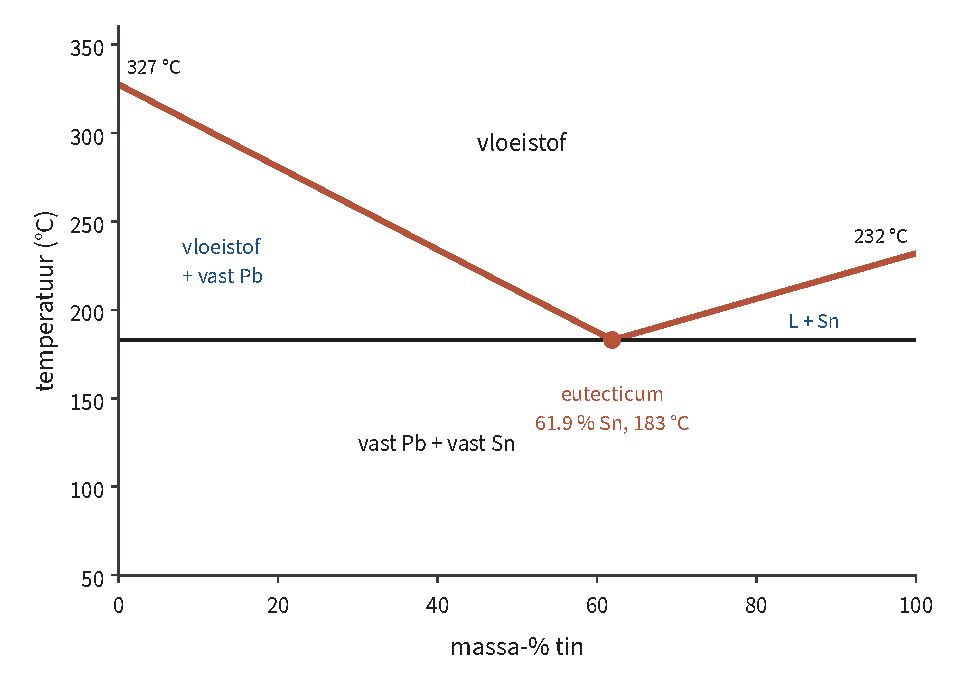
\includegraphics[width=0.7\linewidth]{Figuren/eutecticum}
    \caption{Vereenvoudigd eutectisch diagram van lood--tin (de beperkte vaste oplosbaarheid aan beide kanten is weggelaten). De liquiduslijnen dalen vanuit de smeltpunten van lood (\SI{327}{\celsius}) en tin (\SI{232}{\celsius}) tot het eutecticum bij \num{61.9}~massaprocent tin en \SI{183}{\celsius}.}
    \label{fig:eutecticum}
\end{figure}

Typische voorbeelden:
\begin{itemize}
\item Lood--tin (Pb--Sn) met eutecticum bij \num{61.9}~massaprocent tin ($x_{\text{Sn}} = 0.74$) en $T = \SI{183}{\celsius}$: de basis van klassiek soldeertin. Omdat lood giftig is, gebruikt men vandaag tin--zilver--koperlegeringen die rond \SI{217}{\celsius} smelten.
\item Koper--zilver (Cu--Ag) met eutecticum bij \num{71.9}~massaprocent zilver en $T = \SI{779}{\celsius}$ (zilversoldeer).
\item Natriumchloride--water ($\mathrm{NaCl}$--$\mathrm{H_2O}$) met eutecticum bij \SI{-21}{\celsius}, gebruikt als koudemiddel.
\end{itemize}

\subsubsection{Vriespuntsverlaging}
\label{sec:vriespuntsverlaging}

Voor een verdunde oplossing kan de verlaging van het vriespunt van het oplosmiddel direct uit de chemische potentiaal worden afgeleid. Voor een ideale verdunde oplossing geldt:
\begin{equation}
\Delta T_f = K_f \cdot m,
\end{equation}
waarin $K_f$ de cryoscopische constante (voor water $K_f = \SI{1.86}{\kelvin\kilogram\per\mole}$) en $m$ de molaliteit van de opgeloste stof is. Deze colligatieve eigenschap behoort, samen met dampdrukverlaging, kookpuntsverhoging en osmotische druk, tot de vier eigenschappen die hierna worden samengevat.

\subsection{Colligatieve eigenschappen}
\label{sec:colligatief}

De aanwezigheid van een opgeloste component be\"invloedt het fase-evenwicht van het oplosmiddel op vier verwante manieren. Deze \emph{colligatieve eigenschappen} zijn allen een gevolg van de daling van de chemische potentiaal van het oplosmiddel door menging (vergelijking~\eqref{eq:mu-mengsel-ideaal}): zij hangen daardoor enkel af van het \emph{aantal} opgeloste deeltjes, niet van hun chemische aard.

\begin{enumerate}
\item \textbf{Dampdrukverlaging} (Raoult): $p = x_{\text{oplm}}\,p^*_{\text{oplm}}$.
\item \textbf{Kookpuntsverhoging}: $\Delta T_b = K_b \cdot m$ (voor water: $K_b = \SI{0.512}{\kelvin\kilogram\per\mole}$).
\item \textbf{Vriespuntsverlaging}: $\Delta T_f = -K_f \cdot m$ (\S~\ref{sec:vriespuntsverlaging}).
\item \textbf{Osmotische druk}: $\Pi = c R T$ (vergelijking van Van 't Hoff).
\end{enumerate}

\begin{voorbeeld}{Osmotische druk van een fysiologische zoutoplossing}
Een fysiologische zoutoplossing bevat \SI{9}{\gram\per\litre} NaCl. Met $M_{\mathrm{NaCl}} = \SI{58.4}{\gram\per\mole}$ volgt $c \approx 2 \cdot \SI{0.154}{\mole\per\litre} = \SI{0.308}{\mole\per\litre}$ (factor 2 wegens dissociatie in $\mathrm{Na^+}$ en $\mathrm{Cl^-}$). Bij \SI{310}{\kelvin} (lichaamstemperatuur) bedraagt de osmotische druk:
\[
\Pi = (\SI{308}{\mole\per\metre\cubed})(\SI{8.314}{\joule\per\mole\per\kelvin})(\SI{310}{\kelvin}) \approx \SI{7.9e5}{\pascal} = \SI{7.9}{\bar}.
\]
Vandaar dat bloedcellen in zuiver water zwellen en barsten (hemolyse).
\end{voorbeeld}

\section{Scheidingsprocessen: een thermodynamisch perspectief}
\label{sec:scheidingsprocessen}

De voorbije secties hebben aangetoond dat damp-vloeistofevenwicht, vloeistof-vloeistofevenwicht en vast-vloeistofevenwicht allen voortvloeien uit dezelfde thermodynamische voorwaarde: de gelijkheid van chemische potentialen tussen fasen. Voor de ingenieur vormt dit de theoretische basis van vrijwel alle scheidingsprocessen --- en het sluit rechtstreeks aan bij de industri\"ele toepassingen die reeds in hoofdstuk~\ref{ch:intermoleculair} werden opgesomd.

\begin{itemize}
\item \textbf{Destillatie} berust op het verschil in samenstelling tussen vloeistof en damp bij VLE.
\item \textbf{Vloeistof-vloeistofextractie} berust op de verdeling van een component tussen twee onmengbare vloeistoffasen (Nernst, \S~\ref{sec:nernst}).
\item \textbf{Kristallisatie} berust op SLE en het uitkristalliseren van een component bij afkoeling.
\item \textbf{Absorptie} en \textbf{desorptie} berusten op de oplosbaarheid van gassen in vloeistoffen (Henry, \S~\ref{sec:henry}).
\item \textbf{Droging} berust op de evenwichtsdampdruk boven een vaste stof of vloeistof (Clausius--Clapeyron, Antoine).
\item \textbf{Omgekeerde osmose} berust op het overwinnen van de osmotische druk door uitwendige arbeid.
\end{itemize}

In alle gevallen geldt: de thermodynamica bepaalt de maximale haalbare scheiding. De procestechnologie bepaalt hoe dicht een werkelijk proces deze grens kan benaderen. Deze voorbeelden zullen in een vervolgcursus Scheidingstechnologie uitgebreid aan bod komen.

\section{Samenvatting en reflectie}

\begin{samenvatting}{Fase-evenwicht in niet-reagerende systemen}
\begin{itemize}
\item Evenwichtsvoorwaarde: voor elke component is de chemische potentiaal gelijk in alle fasen. De fasenregel $F = C - P + 2$ telt de vrije variabelen.
\item Zuivere stof: Clapeyron $\dd p/\dd T = \Delta H/(T\Delta V)$; voor verdampen Clausius--Clapeyron en in de praktijk Antoine. Het $p$--$T$-fasediagram toont tripelpunt en kritisch punt.
\item Ideale mengsels: wet van Raoult $p_i = x_i p_i^*$. Bubbelpunt $P = \sum x_i p_i^*$, dampsamenstelling $y_i = x_i p_i^*/P$, relatieve vluchtigheid $\alpha = p_A^*/p_B^*$.
\item VLE-diagrammen ($P$--$x$--$y$, $T$--$x$--$y$, $x$--$y$) stel je zelf op met Raoult en Antoine. De hefboomwet geeft de verhouding vloeistof/damp.
\item Re\"ele mengsels: $a_i = \gamma_i x_i$; positieve en negatieve afwijkingen kunnen leiden tot azeotropen.
\item Verdunde opgeloste stoffen en gassen: wet van Henry $p_i = x_i H_i$. Let op de eenheden; gassen lossen slechter op bij hogere temperatuur.
\item Vloeistof-vloeistofevenwicht: verdelingswet van Nernst; ternaire diagrammen met binodale curve, bindlijnen en hefboomwet.
\item Vast-vloeistof: eutectische diagrammen en colligatieve eigenschappen (vriespuntsdaling, kookpuntsverhoging, osmotische druk).
\end{itemize}
\end{samenvatting}

\begin{reflectie}{Fase-evenwicht in niet-reagerende systemen}
\begin{enumerate}
\item Waarom kookt water in de bergen bij een lagere temperatuur, en waarom duurt het daar langer om een ei te koken?
\item Waarom is de bubbelpuntlijn in een $P$--$x$--$y$-diagram van een ideaal mengsel een rechte, en de dauwpuntlijn niet?
\item Wat gebeurt er met de samenstelling van de vloeistof die achterblijft in een ketel waarin je een benzeen--tolueenmengsel laat koken?
\item Waarom kun je door gewone destillatie geen ethanol zuiverder dan 95.6\,\% maken?
\item Waarom geldt voor het oplosmiddel de wet van Raoult en voor de opgeloste stof de wet van Henry, in dezelfde oplossing?
\item Waarom bruist een fles spuitwater meer als ze warm is?
\item Hoe lees je in een ternair diagram af hoeveel aceton er in het extract zit, en waarom moet het mengpunt binnen de binodale curve liggen om te kunnen extraheren?
\end{enumerate}
\end{reflectie}

Fase-evenwicht en chemisch evenwicht berusten op hetzelfde criterium: de Gibbs-energie is minimaal, of anders gezegd, de chemische potentialen zijn in evenwicht. In hoofdstuk~\ref{ch:reagerend} passen we dit criterium toe op systemen waarin de componenten ook met elkaar reageren.



\newpage
\section{Oefeningen}

% Oefeningen bij dit hoofdstuk (ingevoegd achteraan het hoofdstuk met \input).
% Een oefening:  \begin{oefening} ... \end{oefening}   (boek en website)
% De oplossing:  \begin{oplossing} ... \end{oplossing}       (enkel website, dichtgeklapt)

Neem $R = \SI{8.314}{\joule\per\mole\per\kelvin}$, $\SI{1}{\bar} = \SI{e5}{\pascal}$ en $\SI{760}{mmHg} = \SI{1.01325}{\bar}$.

\begin{oefening}\label{oef:h5-1}
Voor water geldt de Antoine-vergelijking \(\log_{10} p = A - B/(T + C)\) met \(A = 8.07131\), \(B = 1730.63\), \(C = 233.426\), waarbij \(p\) in mmHg en \(T\) in °C (geldig van \(1\) tot \(100\,^\circ\mathrm{C}\)).

\begin{enumerate}
\item[(a)]
  Bereken de dampdruk van water bij \(50\), \(80\) en \(120\,^\circ\mathrm{C}\), in mbar.
\item[(b)]
  Schat dezelfde dampdrukken met de vergelijking van Clausius--Clapeyron, vertrekkend van het normale kookpunt (\(1.013\,\mathrm{bar}\) bij \(100\,^\circ\mathrm{C}\)) met \(\Delta H_{\text{vap}} = 40.7\,\mathrm{kJ/mol}\).
\item[(c)]
  Verklaar de verschillen. Welke waarde bij \(120\,^\circ\mathrm{C}\) vertrouw je het meest?
\end{enumerate}
\end{oefening}
\begin{oplossing}
\textbf{Resultaat:} (a) Antoine: \textbf{123 mbar}, \textbf{473 mbar} en \textbf{1993 mbar}. (b) Clausius--Clapeyron: \textbf{133 mbar}, \textbf{482 mbar} en \textbf{1975 mbar}. (c) Clausius--Clapeyron wijkt tot 8 \% af omdat \(\Delta H_{\text{vap}}\) niet constant is.

\textbf{(a)} Bij \(50\,^\circ\mathrm{C}\):

\[
\log_{10} p = 8.07131 - \frac{1730.63}{50 + 233.426} = 1.965 \quad\Rightarrow\quad p = 92.3\,\mathrm{mmHg} = 123\,\mathrm{mbar}
\]

Op dezelfde manier: \(354.5\,\mathrm{mmHg} = 473\,\mathrm{mbar}\) bij \(80\,^\circ\mathrm{C}\) en \(1495\,\mathrm{mmHg} = 1993\,\mathrm{mbar}\) bij \(120\,^\circ\mathrm{C}\). Controleer eerst de eenheden met een bekend punt: bij \(100\,^\circ\mathrm{C}\) geeft de vergelijking \(760\,\mathrm{mmHg}\).

\textbf{(b)} Bij \(50\,^\circ\mathrm{C}\):

\[
\ln\frac{p_2}{1.013\,\mathrm{bar}} = -\frac{40\,700}{8.314}\left(\frac{1}{323.15} - \frac{1}{373.15}\right) = -2.03 \quad\Rightarrow\quad p_2 = 0.133\,\mathrm{bar}
\]

Bij \(80\,^\circ\mathrm{C}\) en \(120\,^\circ\mathrm{C}\) vind je \(482\) en \(1975\,\mathrm{mbar}\).

\textbf{(c)} De experimentele waarden zijn \(123\), \(474\) en \(1985\,\mathrm{mbar}\). Antoine is een empirische fit en is binnen het geldigheidsgebied zeer nauwkeurig. Clausius--Clapeyron veronderstelt een constante \(\Delta H_{\text{vap}}\), terwijl die bij lagere temperatuur groter is (\(43.0\,\mathrm{kJ/mol}\) bij \(50\,^\circ\mathrm{C}\)): hoe verder van het referentiepunt, hoe groter de fout. Bij \(120\,^\circ\mathrm{C}\) ligt de temperatuur buiten het geldigheidsgebied van deze Antoine-parameters, maar dicht bij het referentiepunt van Clausius--Clapeyron: beide schattingen liggen binnen 1 \% van de werkelijkheid. Dit is de druk in een snelkookpan of een stoomsterilisator (autoclaaf).
\end{oplossing}

\begin{oefening}\label{oef:h5-2}
Een vloeibaar mengsel van \(n\)-hexaan (A) en \(n\)-octaan (B) met \(x_A = 0.30\) bevindt zich bij \(80\,^\circ\mathrm{C}\). De verzadigingsdampdrukken bedragen \(p_A^* = 1.42\,\mathrm{bar}\) en \(p_B^* = 0.23\,\mathrm{bar}\). Behandel het mengsel als ideaal.

\begin{enumerate}
\item[(a)]
  Bereken de bubbelpuntdruk.
\item[(b)]
  Bereken de samenstelling van de eerste dampbel.
\item[(c)]
  Bereken de relatieve vluchtigheid \(\alpha_{AB}\) en beoordeel hoe moeilijk de scheiding door destillatie is.
\end{enumerate}
\end{oefening}
\begin{oplossing}
\textbf{Resultaat:} (a) \(P\) = \textbf{0.587 bar}. (b) \(y_A\) = \textbf{0.726}, \(y_B\) = 0.274. (c) \(\alpha_{AB}\) = \textbf{6.2}: zeer eenvoudige scheiding.

\textbf{(a)} Volgens Raoult:

\[
P = x_A p_A^* + x_B p_B^* = (0.30)(1.42) + (0.70)(0.23) = 0.426 + 0.161 = 0.587\,\mathrm{bar}
\]

\textbf{(b)} \(y_A = x_A p_A^*/P = 0.426/0.587 = 0.726\) en \(y_B = 0.274\). De damp bevat meer dan dubbel zoveel hexaan als de vloeistof.

\textbf{(c)} \(\alpha_{AB} = p_A^*/p_B^* = 1.42/0.23 = 6.2\). Met \(\alpha \geq 5\) is de scheiding zeer eenvoudig: een kolom met weinig schotels volstaat. Ter vergelijking: benzeen--tolueen (\(\alpha = 2.5\)) vraagt al meer schotels, en voor isomeren met \(\alpha \approx 1.1\) zijn kolommen van honderd schotels nodig.
\end{oplossing}

\begin{oefening}
In een flashvat wordt een hexaan--octaanmengsel met globale samenstelling \(z_A = 0.50\) gebracht op \(80\,^\circ\mathrm{C}\) en de druk van Oefening~\ref{oef:h5-2} (\(0.587\,\mathrm{bar}\)). Bij die temperatuur en druk zijn de vloeistof en de damp in evenwicht met de samenstellingen uit Oefening~\ref{oef:h5-2}.

\begin{enumerate}
\item[(a)]
  Waarom splitst dit mengsel in twee fasen?
\item[(b)]
  Bereken de verhouding \(n_L/n_V\) en de hoeveelheden vloeistof en damp per mol voeding.
\item[(c)]
  Hoeveel hexaan zit in de dampstroom, uitgedrukt als fractie van het hexaan in de voeding?
\end{enumerate}
\end{oefening}
\begin{oplossing}
\textbf{Resultaat:} (a) \(x_A = 0.30 < z_A < y_A = 0.726\): tweefasengebied. (b) \(n_L/n_V\) = \textbf{1.13}; \textbf{0.53 mol} vloeistof en \textbf{0.47 mol} damp. (c) \textbf{68 \%} van het hexaan gaat naar de damp.

\textbf{(a)} Bij deze \(T\) en \(P\) ligt de bubbelpuntcurve bij \(x_A = 0.30\) en de dauwpuntcurve bij \(y_A = 0.726\). Een globale samenstelling daartussen valt in het tweefasengebied: het mengsel valt uiteen in een vloeistof met \(x_A = 0.30\) en een damp met \(y_A = 0.726\).

\textbf{(b)}

\[
\frac{n_L}{n_V} = \frac{y_A - z_A}{z_A - x_A} = \frac{0.726 - 0.50}{0.50 - 0.30} = 1.13
\]

Per mol voeding: \(n_L = 1.13/2.13 = 0.53\,\mathrm{mol}\) en \(n_V = 0.47\,\mathrm{mol}\).

\textbf{(c)} Hexaan in de damp: \((0.47)(0.726) = 0.341\,\mathrm{mol}\), van de \(0.50\,\mathrm{mol}\) in de voeding, dus \(68\,\%\). Eén evenwichtstrap geeft een gedeeltelijke scheiding; een destillatiekolom zet zulke trappen in serie. Dit is precies de basis van de McCabe--Thiele-methode in de cursus Scheidingstechnologie.
\end{oplossing}

\begin{oefening}
Voorspel voor de volgende binaire mengsels of ze zich ongeveer ideaal gedragen, een positieve afwijking van Raoult vertonen (met mogelijk een minimaal kokende azeotroop) of een negatieve afwijking (met mogelijk een maximaal kokende azeotroop). Gebruik de intermoleculaire krachten uit hoofdstuk~\ref{ch:intermoleculair}.

\begin{enumerate}
\item[(a)]
  benzeen--tolueen,
\item[(b)]
  \(n\)-hexaan--ethanol,
\item[(c)]
  salpeterzuur--water.
\end{enumerate}

Waarom kan je met gewone destillatie geen zuivere ethanol maken, en hoe maakt de industrie toch watervrije bio-ethanol voor benzine (E10)?
\end{oefening}
\begin{oplossing}
\textbf{Resultaat:} (a) \textbf{Bijna ideaal}, geen azeotroop. (b) \textbf{Positieve afwijking}: minimaal kokende azeotroop. (c) \textbf{Negatieve afwijking}: maximaal kokende azeotroop. Ethanol--water vormt een azeotroop bij 95.6 massa-\%; men droogt verder met \textbf{moleculaire zeven} of azeotrope/extractieve destillatie.

\textbf{(a)} Benzeen en tolueen zijn beide apolaire aromaten met vergelijkbare grootte en enkel dispersiekrachten. De interacties A--B zijn ongeveer even sterk als A--A en B--B: het mengsel volgt de wet van Raoult goed (\(\gamma \approx 1\)) en vormt geen azeotroop.

\textbf{(b)} Ethanol vormt waterstofbruggen met zichzelf. Hexaan kan die niet vervangen: elke hexaanmolecule tussen de ethanolmoleculen breekt bruggen zonder er iets sterks voor terug te geven. De interacties A--B zijn zwakker dan A--A en B--B, de moleculen ontsnappen gemakkelijker (\(\gamma > 1\)) en de dampdruk ligt boven Raoult. Hexaan en ethanol vormen een minimaal kokende azeotroop (rond \(59\,^\circ\mathrm{C}\), lager dan beide kookpunten).

\textbf{(c)} Salpeterzuur en water interageren zeer sterk: waterstofbruggen en zelfs gedeeltelijke ionisatie (\(\mathrm{HNO_3 + H_2O \rightarrow H_3O^+ + NO_3^-}\)). A--B is sterker dan A--A en B--B, de dampdruk ligt onder Raoult (\(\gamma < 1\)) en er ontstaat een maximaal kokende azeotroop (ongeveer \(68\,\%\) \(\mathrm{HNO_3}\) in massa, \(120\,^\circ\mathrm{C}\)). Daarom is geconcentreerd salpeterzuur in de handel typisch \(65\)--\(68\,\%\).

\textbf{Ethanol:} bij de azeotrope samenstelling hebben damp en vloeistof dezelfde samenstelling, dus een extra destillatietrap verandert niets meer. Om voorbij \(95.6\,\%\) te geraken, moet men het evenwicht omzeilen: adsorptie van water op een moleculaire zeef (zeoliet 3A, die enkel de kleine watermoleculen binnenlaat), drukwisseldestillatie, of een hulpstof toevoegen die het VLE wijzigt (azeotrope of extractieve destillatie).
\end{oplossing}

\begin{oefening}
Boven een ethanol--watermengsel met \(x_{\text{EtOH}} = 0.10\) meet men bij \(25\,^\circ\mathrm{C}\) een partiële dampdruk van ethanol van \(24\,\mathrm{mbar}\). De dampdruk van zuivere ethanol bij \(25\,^\circ\mathrm{C}\) bedraagt \(78.7\,\mathrm{mbar}\).

\begin{enumerate}
\item[(a)]
  Bereken de activiteit en de activiteitscoëfficiënt van ethanol.
\item[(b)]
  Is dit een positieve of een negatieve afwijking van Raoult? Is dat in overeenstemming met de azeotroop van ethanol--water?
\item[(c)]
  Bepaal de parameter \(A\) van het Margules-éénparametermodel en voorspel daarmee \(\gamma_{\text{EtOH}}\) bij \(x = 0.50\) en bij oneindige verdunning.
\item[(d)]
  Waarom ruik je alcohol in een glas wijn (12 vol-\%, \(x \approx 0.04\)) veel sterker dan je met Raoult zou verwachten?
\end{enumerate}
\end{oefening}
\begin{oplossing}
\textbf{Resultaat:} (a) \(a\) = 0.305, \(\gamma\) = \textbf{3.05}. (b) \textbf{Positieve} afwijking, consistent met een minimaal kokende azeotroop. (c) \(A\) = \textbf{1.38}; \(\gamma(0.5)\) = \textbf{1.41} en \(\gamma^\infty\) = \textbf{3.96}. (d) Ethanol ontsnapt bij lage concentratie bijna 4 keer gemakkelijker dan volgens Raoult.

\textbf{(a)} Met \(p_i = a_i p_i^* = \gamma_i x_i p_i^*\):

\[
a = \frac{24}{78.7} = 0.305, \qquad \gamma = \frac{a}{x} = \frac{0.305}{0.10} = 3.05
\]

\textbf{(b)} \(\gamma > 1\): positieve afwijking. Ethanol--ethanol en water--water vormen sterke waterstofbrugnetwerken; de apolaire ethylgroep verstoort het netwerk van water. Gemengd zijn de moleculen minder goed `vastgehouden' dan in de zuivere stoffen. Een voldoende grote positieve afwijking geeft een minimaal kokende azeotroop, precies wat ethanol--water vertoont.

\textbf{(c)} Met \(\ln \gamma_A = A x_B^2\):

\[
A = \frac{\ln 3.05}{(0.90)^2} = \frac{1.115}{0.81} = 1.38
\]

Bij \(x = 0.50\): \(\gamma = \exp(1.38 \times 0.25) = 1.41\). Bij oneindige verdunning (\(x_B \to 1\)): \(\gamma^\infty = e^{A} = 3.96\). De literatuurwaarde ligt rond \(4.5\)--\(5\); het symmetrische éénparametermodel is voor dit asymmetrische mengsel slechts een benadering, en daarom gebruikt men in de praktijk Wilson of NRTL.

\textbf{(d)} Bij lage concentratie is \(\gamma \approx \gamma^\infty \approx 4\) à \(5\): de partiële dampdruk van ethanol boven wijn is vier tot vijf keer groter dan Raoult voorspelt. Hetzelfde effect maakt het mogelijk aroma's en alcohol uit verdunde waterige stromen te strippen, en verklaart waarom de eerste fractie bij het distilleren van wijn al sterk alcoholisch is.
\end{oplossing}

\begin{oefening}
Een waterige afvalstroom bevat \(0.050\,\mathrm{mol/L}\) benzoëzuur (conserveermiddel E210). De verdelingscoëfficiënt tussen tolueen en water bedraagt \(K_D = c_{\text{tol}}/c_{\text{water}} = 12\). Men extraheert \(1.0\,\mathrm{L}\) waterige oplossing met tolueen.

\begin{enumerate}
\item[(a)]
  Bereken de resterende concentratie in het water na één extractie met \(0.50\,\mathrm{L}\) tolueen, en het percentage dat verwijderd is.
\item[(b)]
  Hoeveel opeenvolgende extracties met telkens \(0.50\,\mathrm{L}\) vers tolueen zijn nodig om minstens \(99\,\%\) te verwijderen?
\item[(c)]
  Vergelijk één extractie met \(0.50\,\mathrm{L}\) met twee extracties met elk \(0.25\,\mathrm{L}\). Wat besluit je?
\end{enumerate}
\end{oefening}
\begin{oplossing}
\textbf{Resultaat:} (a) \(c\) = \textbf{7.1\ensuremath{\cdot{}}10\ensuremath{^{-3}} mol/L}; \textbf{85.7 \%} verwijderd. (b) \textbf{3 extracties} (2.4 is theoretisch nodig). (c) Twee keer \(0.25\,\mathrm{L}\) verwijdert \textbf{93.8 \%}: verdeeld extraheren is efficiënter.

\textbf{(a)} Massabalans: \(c_0 V_w = c_w V_w + K_D c_w V_o\), dus

\[
c_w = c_0\frac{V_w}{V_w + K_D V_o} = 0.050 \cdot \frac{1}{1 + 12(0.50)} = \frac{0.050}{7} = 7.1\times10^{-3}\,\mathrm{mol/L}
\]

Er blijft \(1/7 = 14.3\,\%\) achter: \(85.7\,\%\) is verwijderd.

\textbf{(b)} Na \(n\) stappen blijft \((1/7)^n\) over. \((1/7)^n \leq 0.01\) geeft \(n \geq \ln 100/\ln 7 = 2.37\), dus drie extracties (na drie stappen blijft \(0.29\,\%\) over).

\textbf{(c)} Per stap met \(0.25\,\mathrm{L}\) blijft \(1/(1 + 12 \times 0.25) = 1/4\) over; na twee stappen \(1/16 = 6.25\,\%\). Met dezelfde totale hoeveelheid oplosmiddel verwijdert men \(93.8\,\%\) in plaats van \(85.7\,\%\). Meerdere kleine extracties (of een tegenstroomkolom) zijn efficiënter dan één grote, een principe dat je ook toepast bij het spoelen van een maatbeker of bij het zetten van thee in twee keer.
\end{oplossing}

\begin{oefening}
Zeewater bevat ongeveer \(0.55\,\mathrm{mol/L}\) opgeloste zouten, hoofdzakelijk NaCl, dat volledig dissocieert.

\begin{enumerate}
\item[(a)]
  Bereken de osmotische druk van zeewater bij \(25\,^\circ\mathrm{C}\).
\item[(b)]
  Welke druk moet een installatie voor omgekeerde osmose minstens leveren om zuiver water te produceren?
\item[(c)]
  Bereken de minimale arbeid om \(1\,\mathrm{m^3}\) zuiver water te winnen, in kWh. Een moderne installatie verbruikt ongeveer \(3\,\mathrm{kWh/m^3}\). Waarom is dat meer?
\item[(d)]
  Waarom mag je als schipbreukeling geen zeewater drinken?
\end{enumerate}
\end{oefening}
\begin{oplossing}
\textbf{Resultaat:} (a) \(\Pi\) = \textbf{27 bar}. (b) Meer dan \textbf{27 bar} (in de praktijk 55--70 bar). (c) \(W_{\min}\) = \textbf{0.76 kWh/m\ensuremath{^{3}}}. (d) Zeewater is \textbf{hypertoon}: het onttrekt water aan je cellen.

\textbf{(a)} Elk mol NaCl geeft twee ionen, dus \(c = 1.10\,\mathrm{mol/L} = 1100\,\mathrm{mol/m^3}\):

\[
\Pi = cRT = (1100)(8.314)(298.15) = 2.73\times10^{6}\,\mathrm{Pa} = 27\,\mathrm{bar}
\]

\textbf{(b)} Om water door het membraan van de zoute naar de zoete kant te persen, moet de uitwendige druk groter zijn dan \(\Pi\). Omdat het zeewater tijdens het proces steeds zouter wordt (het concentraat), werken installaties in de praktijk bij \(55\)--\(70\,\mathrm{bar}\).

\textbf{(c)} De minimale arbeid is de arbeid om een volume \(V\) tegen de osmotische druk in te persen:

\[
W_{\min} = \Pi V = (2.73\times10^{6}\,\mathrm{Pa})(1\,\mathrm{m^3}) = 2.73\,\mathrm{MJ} = 0.76\,\mathrm{kWh}
\]

Dit is dezelfde ondergrens als de Gibbs-vrije energie van ontmenging (hoofdstuk~\ref{ch:spontaniteit}). Echte installaties verbruiken vier keer meer: de druk moet boven \(\Pi\) liggen om een redelijk debiet te krijgen, het concentraat wordt zouter, en pompen en membranen hebben verliezen (irreversibiliteiten). Toch is omgekeerde osmose veel zuiniger dan verdampen: om \(1\,\mathrm{m^3}\) water te verdampen is ongeveer \(630\,\mathrm{kWh}\) warmte nodig.

\textbf{(d)} Bloed heeft een osmotische druk van ongeveer \(7.9\,\mathrm{bar}\) (zie het voorbeeld van de fysiologische zoutoplossing), zeewater \(27\,\mathrm{bar}\). De nieren kunnen urine maken die hoogstens ongeveer zo zout is als zeewater, zodat ze meer water nodig hebben om het zout uit te scheiden dan je ermee binnenkrijgt. Je droogt uit.
\end{oplossing}

\begin{oefening}
De \emph{relatieve vochtigheid} van lucht is de verhouding van de partiële waterdampdruk tot de dampdruk van water bij dezelfde temperatuur: \(\mathrm{RV} = p_{\mathrm{H_2O}}/p^*_{\mathrm{H_2O}}(T)\). Gebruik de Antoine-vergelijking van Oefening~\ref{oef:h5-1}.

\begin{enumerate}
\item[(a)]
  In een klaslokaal is het \(22\,^\circ\mathrm{C}\) bij een relatieve vochtigheid van \(50\,\%\). Bereken de partiële waterdampdruk.
\item[(b)]
  Bereken het dauwpunt: de temperatuur waarbij die lucht verzadigd raakt en condens vormt.
\item[(c)]
  Leg uit waarom een flesje uit de koelkast (\(5\,^\circ\mathrm{C}\)) in dit lokaal beslaat, en waarom je bril beslaat als je in de winter binnenkomt.
\item[(d)]
  Buitenlucht van \(0\,^\circ\mathrm{C}\) met \(90\,\%\) relatieve vochtigheid wordt binnen opgewarmd tot \(21\,^\circ\mathrm{C}\), zonder water toe te voegen. Bereken de nieuwe relatieve vochtigheid. Waarom is binnenlucht in de winter zo droog?
\end{enumerate}
\end{oefening}
\begin{oplossing}
\textbf{Resultaat:} (a) \(p_{\mathrm{H_2O}}\) = \textbf{13.2 mbar}. (b) Dauwpunt \ensuremath{\approx{}} \textbf{11 °C}. (c) Elk oppervlak kouder dan 11 °C beslaat. (d) RV daalt tot ongeveer \textbf{22 \%}.

\textbf{(a)} Antoine bij \(22\,^\circ\mathrm{C}\): \(\log_{10}p^* = 8.07131 - 1730.63/255.426 = 1.296\), dus \(p^* = 19.8\,\mathrm{mmHg} = 26.3\,\mathrm{mbar}\). Met \(\mathrm{RV} = 0.50\): \(p_{\mathrm{H_2O}} = 13.2\,\mathrm{mbar}\).

\textbf{(b)} Het dauwpunt is de temperatuur waarbij \(p^*(T) = 13.2\,\mathrm{mbar} = 9.88\,\mathrm{mmHg}\). Antoine omvormen:

\[
T = \frac{B}{A - \log_{10}p} - C = \frac{1730.63}{8.07131 - 0.995} - 233.426 = 11.1\,^\circ\mathrm{C}
\]

\textbf{(c)} De lucht vlak tegen een oppervlak van \(5\,^\circ\mathrm{C}\) koelt af onder het dauwpunt. De partiële waterdampdruk (\(13.2\,\mathrm{mbar}\)) is dan groter dan de dampdruk van water bij \(5\,^\circ\mathrm{C}\) (\(8.7\,\mathrm{mbar}\)): de damp is oververzadigd en condenseert. Een bril die buiten op \(0\,^\circ\mathrm{C}\) was, beslaat om dezelfde reden. Dauw op het gras en condens op koude muren (schimmel!) ontstaan zo ook.

\textbf{(d)} Buiten: \(p_{\mathrm{H_2O}} = 0.90 \times p^*(0\,^\circ\mathrm{C}) = 0.90 \times 6.0 = 5.4\,\mathrm{mbar}\). Binnen is \(p^*(21\,^\circ\mathrm{C}) = 24.7\,\mathrm{mbar}\), dus \(\mathrm{RV} = 5.4/24.7 = 22\,\%\). De absolute hoeveelheid water verandert niet, maar warme lucht kan veel meer waterdamp bevatten. Daarom voelt verwarmde winterlucht droog aan en gebruiken sommige mensen een luchtbevochtiger.
\end{oplossing}

\begin{oefening}
Om wegen ijsvrij te houden, strooit men NaCl (\(M = 58.44\,\mathrm{g/mol}\)). Gebruik \(K_f = 1.86\,\mathrm{K\,kg/mol}\) voor water en veronderstel volledige dissociatie en een ideale verdunde oplossing.

\begin{enumerate}
\item[(a)]
  Hoeveel gram NaCl per kg water is nodig om het vriespunt te verlagen tot \(-5\,^\circ\mathrm{C}\)?
\item[(b)]
  Waarom telt elk mol NaCl dubbel? Hoeveel \(\mathrm{CaCl_2}\) (\(M = 111.0\,\mathrm{g/mol}\)) zou je per kg water nodig hebben voor hetzelfde effect?
\item[(c)]
  Waarom heeft strooien bij \(-25\,^\circ\mathrm{C}\) geen zin meer met NaCl?
\end{enumerate}
\end{oefening}
\begin{oplossing}
\textbf{Resultaat:} (a) \textbf{79 g NaCl} per kg water. (b) Colligatief: het aantal deeltjes telt; \textbf{100 g CaCl\ensuremath{_{2}}} (3 ionen per formule-eenheid). (c) Onder het \textbf{eutecticum van \ensuremath{-}21 °C} bevriest de pekel volledig.

\textbf{(a)} De vereiste molaliteit aan opgeloste deeltjes is \(m = \Delta T_f/K_f = 5/1.86 = 2.69\,\mathrm{mol/kg}\). Elk NaCl geeft twee ionen, dus \(1.34\,\mathrm{mol}\) NaCl per kg water, of \((1.34)(58.44) = 79\,\mathrm{g}\).

\textbf{(b)} Vriespuntsverlaging is een colligatieve eigenschap: ze hangt enkel af van het aantal opgeloste deeltjes, omdat elk deeltje de chemische potentiaal van het water evenveel verlaagt. \(\mathrm{CaCl_2}\) geeft drie ionen: \(2.69/3 = 0.896\,\mathrm{mol}\), of \((0.896)(111.0) = 99.5 \approx 100\,\mathrm{g}\) per kg water. Per gram is NaCl dus iets efficiënter, maar \(\mathrm{CaCl_2}\) werkt tot lagere temperaturen (eutecticum \(-50\,^\circ\mathrm{C}\)) en lost exotherm op.

\textbf{(c)} Het eutectisch punt van NaCl--water ligt bij \(-21\,^\circ\mathrm{C}\). Daaronder is geen vloeibare pekel meer stabiel, hoeveel zout je ook toevoegt: ijs en vast zout coëxisteren. In werkelijkheid werkt NaCl al slecht onder ongeveer \(-10\,^\circ\mathrm{C}\), omdat het zout eerst moet oplossen in een dun laagje water. In Scandinavië en Canada gebruikt men dan zand of \(\mathrm{CaCl_2}\).
\end{oplossing}

\begin{oefening}\label{oef:h5-10}
De Henry-constante van zuurstof in water (molfractieschaal) bedraagt \(H = 3.27\times10^{4}\,\mathrm{bar}\) bij \(10\,^\circ\mathrm{C}\) en \(4.26\times10^{4}\,\mathrm{bar}\) bij \(25\,^\circ\mathrm{C}\). Lucht bevat \(21\,\%\) zuurstof; de totale druk is \(1.0\,\mathrm{bar}\). Water bevat \(55.5\,\mathrm{mol}\) per liter.

\begin{enumerate}
\item[(a)]
  Bereken de opgeloste zuurstofconcentratie in mg/L bij beide temperaturen.
\item[(b)]
  Vissen zoals forel hebben minstens ongeveer \(6\,\mathrm{mg/L}\) zuurstof nodig. Wat gebeurt er in een warme zomer, zeker als er ook organisch materiaal afgebroken wordt?
\item[(c)]
  Waarom stijgt de Henry-constante met de temperatuur? Verbind met het teken van de oplosenthalpie en met Le Chatelier.
\end{enumerate}
\end{oefening}
\begin{oplossing}
\textbf{Resultaat:} (a) \textbf{11.4 mg/L} bij 10 °C en \textbf{8.8 mg/L} bij 25 °C. (b) De marge tot de ondergrens van 6 mg/L \textbf{halveert}. (c) Gassen oplossen is \textbf{exotherm}: hogere \(T\) verschuift het evenwicht naar de gasfase.

\textbf{(a)} Met \(p_{\mathrm{O_2}} = 0.21\,\mathrm{bar}\) en \(x = p/H\):

\begin{itemize}
\item
  \(10\,^\circ\mathrm{C}\): \(x = 0.21/3.27\times10^{4} = 6.42\times10^{-6}\), dus \(c = (6.42\times10^{-6})(55.5) = 3.56\times10^{-4}\,\mathrm{mol/L} = 11.4\,\mathrm{mg/L}\).
\item
  \(25\,^\circ\mathrm{C}\): \(x = 4.93\times10^{-6}\), dus \(c = 2.74\times10^{-4}\,\mathrm{mol/L} = 8.8\,\mathrm{mg/L}\).
\end{itemize}

De gemeten waarden zijn \(11.3\) en \(8.3\,\mathrm{mg/L}\).

\textbf{(b)} Bij \(25\,^\circ\mathrm{C}\) is de evenwichtsconcentratie een kwart lager, en de marge boven \(6\,\mathrm{mg/L}\) zakt van \(5.4\) naar \(2.8\,\mathrm{mg/L}\). Tegelijk verbruiken vissen en bacteriën meer zuurstof bij hogere temperatuur (reactiesnelheden stijgen, hoofdstuk~\ref{ch:kinetiek}), en het water is in de zomer vaak trager en minder gemengd. Het resultaat is vissterfte, ook zonder vervuiling. Daarom mogen centrales en industrie hun koelwater niet onbeperkt warm lozen.

\textbf{(c)} Een opgeloste gasmolecule wordt door het water omringd en aangetrokken (dipool--geïnduceerde dipool- en dispersiekrachten, hoofdstuk~\ref{ch:intermoleculair}): oplossen is exotherm. Bij hogere temperatuur schuift het evenwicht naar de endotherme kant, de gasfase. Hetzelfde verklaart waarom lauwe frisdrank sneller verschaalt dan koude.
\end{oplossing}

\begin{oefening}
Een duiker ademt perslucht (\(79\,\%\) \(\mathrm{N_2}\)) op \(30\,\mathrm{m}\) diepte, waar de totale druk \(4.0\,\mathrm{bar}\) bedraagt. Behandel bloed als water (\(55.5\,\mathrm{mol/L}\)) met een Henry-constante voor stikstof van \(H = 9.0\times10^{4}\,\mathrm{bar}\) bij \(37\,^\circ\mathrm{C}\).

\begin{enumerate}
\item[(a)]
  Bereken de concentratie opgeloste stikstof in het bloed aan het oppervlak en op \(30\,\mathrm{m}\) diepte, na verzadiging.
\item[(b)]
  De duiker stijgt veel te snel op. Hoeveel milliliter stikstofgas (bij \(37\,^\circ\mathrm{C}\) en \(1\,\mathrm{bar}\)) komt per liter bloed vrij? Gebruik de ideale gaswet (hoofdstuk~\ref{ch:energie}).
\item[(c)]
  Waarom gebruiken diepzeeduikers helium in plaats van stikstof in hun ademgas?
\end{enumerate}
\end{oefening}
\begin{oplossing}
\textbf{Resultaat:} (a) \textbf{0.49 mmol/L} aan het oppervlak, \textbf{1.95 mmol/L} op 30 m. (b) Ongeveer \textbf{38 mL N\ensuremath{_{2}}} per liter bloed (bijna 0.2 L voor 5 L bloed). (c) Helium lost \textbf{slechter} op en diffundeert sneller.

\textbf{(a)} Met \(x = p_{\mathrm{N_2}}/H\) en \(c = 55.5\,x\):

\begin{itemize}
\item
  Oppervlak: \(p_{\mathrm{N_2}} = 0.79\,\mathrm{bar}\), \(x = 8.8\times10^{-6}\), \(c = 0.49\,\mathrm{mmol/L}\).
\item
  \(30\,\mathrm{m}\): \(p_{\mathrm{N_2}} = 3.16\,\mathrm{bar}\), \(x = 3.5\times10^{-5}\), \(c = 1.95\,\mathrm{mmol/L}\).
\end{itemize}

\textbf{(b)} Bij snel opstijgen komt het overschot \(\Delta c = 1.46\,\mathrm{mmol/L}\) vrij als gas:

\[
V = \frac{nRT}{p} = \frac{(1.46\times10^{-3})(8.314)(310.15)}{1.0\times10^{5}} = 3.8\times10^{-5}\,\mathrm{m^3} = 38\,\mathrm{mL}
\]

Voor \(5\,\mathrm{L}\) bloed is dat bijna \(0.2\,\mathrm{L}\) gas, dat bellen vormt in bloedvaten en gewrichten: de caissonziekte. Het is hetzelfde fenomeen als het bruisen van een fles spuitwater (het voorbeeld van \(\mathrm{CO_2}\) in de theorie). Duikers stijgen daarom langzaam op met decompressiestops, zodat de stikstof via de longen kan ontsnappen.

\textbf{(c)} Helium heeft een nog grotere Henry-constante (het lost slechter op in bloed en vetweefsel) en diffundeert sneller uit het lichaam. Bovendien vermijdt het de verdovende werking van stikstof onder hoge druk (dieptedronkenschap).
\end{oplossing}

\begin{oefening}
Het tripelpunt van \(\mathrm{CO_2}\) ligt bij \(-56.6\,^\circ\mathrm{C}\) en \(5.18\,\mathrm{bar}\); het kritisch punt bij \(31.0\,^\circ\mathrm{C}\) en \(73.8\,\mathrm{bar}\). De sublimatie-enthalpie bedraagt \(25.2\,\mathrm{kJ/mol}\).

\begin{enumerate}
\item[(a)]
  Waarom smelt droog ijs niet bij atmosferische druk, maar sublimeert het?
\item[(b)]
  Bereken met de vergelijking van Clausius--Clapeyron (toegepast op sublimatie) de temperatuur van droog ijs bij \(1.013\,\mathrm{bar}\).
\item[(c)]
  Bij het cafeïnevrij maken van koffie gebruikt men \(\mathrm{CO_2}\) bij \(40\,^\circ\mathrm{C}\) en \(250\,\mathrm{bar}\). In welke toestand bevindt het \(\mathrm{CO_2}\) zich, en waarom is dat voordelig?
\item[(d)]
  In een \(\mathrm{CO_2}\)-brandblusser bij \(20\,^\circ\mathrm{C}\) hoor je vloeistof klotsen. Bij welke druk ongeveer? Waarom kan dat niet in de zomer bij \(35\,^\circ\mathrm{C}\)?
\end{enumerate}
\end{oefening}
\begin{oplossing}
\textbf{Resultaat:} (a) De druk van \textbf{1 bar ligt onder het tripelpunt} (5.18 bar). (b) \(T\) = \textbf{194 K} (\ensuremath{-}79 °C). (c) \textbf{Superkritisch fluïdum}. (d) Ongeveer \textbf{57 bar}; boven 31 °C bestaat \textbf{geen vloeistof} meer.

\textbf{(a)} Vloeibaar \(\mathrm{CO_2}\) is enkel stabiel bij drukken boven het tripelpunt. Bij \(1\,\mathrm{bar}\) grenst het gebied van de vaste stof in het fasediagram rechtstreeks aan dat van het gas: bij opwarmen gaat droog ijs meteen over naar damp. Daarom laat het geen plas na, wat het handig maakt om ijsjes of vaccins koud te houden.

\textbf{(b)} Vertrekkend van het tripelpunt (\(p_1 = 5.18\,\mathrm{bar}\), \(T_1 = 216.55\,\mathrm{K}\)):

\[
\frac{1}{T_2} = \frac{1}{T_1} - \frac{R}{\Delta H_{\text{sub}}}\ln\frac{p_2}{p_1} = \frac{1}{216.55} - \frac{8.314}{25\,200}\ln\frac{1.013}{5.18} = 5.156\times10^{-3}\,\mathrm{K^{-1}}
\]

zodat \(T_2 = 194\,\mathrm{K} = -79\,^\circ\mathrm{C}\) (experimenteel \(-78.5\,^\circ\mathrm{C}\)).

\textbf{(c)} \(40\,^\circ\mathrm{C} > T_c\) en \(250\,\mathrm{bar} > p_c\): het \(\mathrm{CO_2}\) is een superkritisch fluïdum. Het heeft een dichtheid zoals een vloeistof (en lost dus cafeïne goed op), maar een lage viscositeit en hoge diffusiviteit zoals een gas (en dringt dus snel in de bonen). Na de extractie laat men de druk zakken: het \(\mathrm{CO_2}\) wordt een gas en verdwijnt volledig, zonder residu van een toxisch oplosmiddel.

\textbf{(d)} In de fles zijn vloeistof en damp in evenwicht; de druk is de dampdruk van \(\mathrm{CO_2}\) bij \(20\,^\circ\mathrm{C}\), ongeveer \(57\,\mathrm{bar}\). Boven de kritische temperatuur van \(31\,^\circ\mathrm{C}\) kan \(\mathrm{CO_2}\) bij geen enkele druk vloeibaar zijn: de fles bevat dan één superkritische fase en de druk stijgt sterk. Daarom moeten blussers en \(\mathrm{CO_2}\)-flessen voor frisdrankmachines koel bewaard worden.
\end{oplossing}

\begin{oefening}
Een vaak gehoorde verklaring voor het glijden van een schaats is dat de druk onder het ijzer het ijs doet smelten. Controleer die verklaring. Gebruik voor water bij \(0\,^\circ\mathrm{C}\): \(\Delta H_{\text{fus}} = 6.01\,\mathrm{kJ/mol}\), \(V_m(\mathrm{l}) = 18.02\,\mathrm{cm^3/mol}\) en \(V_m(\mathrm{s}) = 19.65\,\mathrm{cm^3/mol}\).

\begin{enumerate}
\item[(a)]
  Bereken \(\mathrm{d}p/\mathrm{d}T\) voor de smeltlijn van water met de vergelijking van Clapeyron. Waarom is het teken negatief?
\item[(b)]
  Een schaatser van \(70\,\mathrm{kg}\) staat op één schaats. Het contactoppervlak bedraagt \(3\,\mathrm{mm} \times 10\,\mathrm{cm}\). Hoeveel daalt het smeltpunt?
\item[(c)]
  Hoe klein zou het contactoppervlak moeten zijn om ijs van \(-10\,^\circ\mathrm{C}\) te laten smelten?
\item[(d)]
  Wat besluit je over de verklaring? Wat is de werkelijke oorzaak?
\end{enumerate}
\end{oefening}
\begin{oplossing}
\textbf{Resultaat:} (a) \(\mathrm{d}p/\mathrm{d}T\) = \textbf{\ensuremath{-}135 bar/K}. (b) Druk 23 bar, smeltpunt \textbf{slechts 0.17 K lager}. (c) Ongeveer \textbf{5 mm\ensuremath{^{2}}} (1350 bar). (d) Drukvorming verklaart het glijden niet. De oorzaak is wrijvingswarmte en een dun vloeibaar laagje dat altijd op ijs aanwezig is.

\textbf{(a)}

\[
\frac{\mathrm{d}p}{\mathrm{d}T} = \frac{\Delta H_{\text{fus}}}{T\,\Delta V_{\text{fus}}} = \frac{6010}{(273.15)(-1.63\times10^{-6})} = -1.35\times10^{7}\,\mathrm{Pa/K} = -135\,\mathrm{bar/K}
\]

Het teken is negatief omdat ijs een groter volume heeft dan vloeibaar water (\(\Delta V_{\text{fus}} < 0\)), door het open waterstofbrugnetwerk. Water is een van de weinige stoffen waarbij druk het smeltpunt verlaagt.

\textbf{(b)} \(p = F/A = (70)(9.81)/(3\times10^{-4}) = 2.3\times10^{6}\,\mathrm{Pa} = 23\,\mathrm{bar}\), zodat \(\Delta T = 23/(-135) = -0.17\,\mathrm{K}\).

\textbf{(c)} Voor \(\Delta T = -10\,\mathrm{K}\) is \(1350\,\mathrm{bar}\) nodig. Dan moet \(A = 687/(1.35\times10^{8}) = 5\times10^{-6}\,\mathrm{m^2} = 5\,\mathrm{mm^2}\), kleiner dan een speldenkop voor een volwassene.

\textbf{(d)} Bij gewone schaatstemperaturen kan druk het ijs niet doen smelten. Je kan bovendien ook schaatsen op ijs van \(-20\,^\circ\mathrm{C}\), en ook met schoenen glijd je uit. Twee andere verschijnselen verklaren het: de wrijving tussen schaats en ijs levert warmte die een dun laagje doet smelten, en het ijsoppervlak draagt zelfs ver onder \(0\,^\circ\mathrm{C}\) een vloeistofachtig laagje van enkele moleculen dik. Voor een auto is het effect nog kleiner: \(1500\,\mathrm{kg}\) op vier banden van elk \(150\,\mathrm{cm^2}\) geeft slechts \(2.5\,\mathrm{bar}\), of \(0.02\,\mathrm{K}\). Deze oefening toont hoe een snelle berekening een populaire verklaring kan weerleggen.
\end{oplossing}

\begin{oefening}
Om oploskoffie te maken wordt koffie-extract ingevroren en daarna onder vacuüm gebracht. Het ijs sublimeert zonder te smelten, zodat de aroma's niet door verhitting verloren gaan. Het tripelpunt van water ligt bij \(273.16\,\mathrm{K}\) en \(611.7\,\mathrm{Pa}\). De sublimatie-enthalpie van ijs bedraagt \(\Delta H_{\text{sub}} = 51.0\,\mathrm{kJ/mol}\).

\begin{enumerate}
\item[(a)]
  Bereken de sublimatiedruk van ijs bij \(-20\,^\circ\mathrm{C}\) en bij \(-40\,^\circ\mathrm{C}\) met de vergelijking van Clausius--Clapeyron.
\item[(b)]
  Onder welke druk moet de vriesdroger werken om het ijs bij \(-20\,^\circ\mathrm{C}\) te laten sublimeren? Waarom mag de druk nooit boven \(611.7\,\mathrm{Pa}\) komen?
\item[(c)]
  Hoeveel energie per kilogram verwijderd water moet worden toegevoerd? Vergelijk met verdampen bij \(100\,^\circ\mathrm{C}\) (\(2257\,\mathrm{kJ/kg}\)).
\item[(d)]
  Waarom bouwt men toch vriesdrogers, ondanks dit hogere energieverbruik?
\end{enumerate}
\end{oefening}
\begin{oplossing}
\textbf{Resultaat:} (a) \textbf{104 Pa} bij \ensuremath{-}20 °C en \textbf{13 Pa} bij \ensuremath{-}40 °C. (b) Onder ongeveer \textbf{100 Pa}, dus 1/1000 van de atmosfeerdruk. Boven het tripelpunt zou het ijs smelten. (c) \textbf{2.83 MJ/kg}, ongeveer 25 \% meer dan verdampen. (d) Kwaliteit: geen verhitting, behoud van aroma en structuur.

\textbf{(a)} Met het tripelpunt als referentie:

\[
\ln\frac{p}{611.7\,\mathrm{Pa}} = -\frac{51\,000}{8.314}\left(\frac{1}{253.15}-\frac{1}{273.16}\right) = -1.77
\]

zodat \(p(-20\,^\circ\mathrm{C}) = 104\,\mathrm{Pa}\) (tabelwaarde \(103\,\mathrm{Pa}\)). Op dezelfde manier is \(p(-40\,^\circ\mathrm{C}) = 13\,\mathrm{Pa}\).

\textbf{(b)} De waterdampdruk boven het product moet lager zijn dan \(104\,\mathrm{Pa}\), anders is er geen netto sublimatie. In de praktijk werkt men bij \(10\) à \(100\,\mathrm{Pa}\) en vangt men de damp op een condensor van ongeveer \(-50\,^\circ\mathrm{C}\). Boven de tripelpuntsdruk bestaat vloeibaar water als stabiele fase, zodat het ijs bij opwarmen zou smelten in plaats van te sublimeren. Dat is precies wat je wil vermijden.

\textbf{(c)} \(51.0/0.018015 = 2830\,\mathrm{kJ/kg}\). Dat is de som van smelt- en verdampingsenthalpie en dus meer dan voor verdampen alleen (\(2257\,\mathrm{kJ/kg}\) bij \(100\,^\circ\mathrm{C}\)). Daar komen nog de energie voor de vacuümpomp en de koeling van de condensor bij.

\textbf{(d)} De vluchtige aroma's van koffie ontbinden of verdampen bij verhitten. Door het water bij lage temperatuur te verwijderen blijft de smaak beter bewaard en houdt het product een poreuze structuur die snel oplost. Om dezelfde reden worden ook vaccins, bloedplasma en astronautenvoeding gevriesdroogd.
\end{oplossing}

\begin{oefening}
Stel het $T$--$x$--$y$-diagram op van een ideaal mengsel van $n$-hexaan (A) en $n$-heptaan (B) bij \SI{1.013}{\bar}. Antoineconstanten ($\log_{10} p^*/\si{mmHg} = A - B/(T/\si{\celsius} + C)$): hexaan $A = 6.87601$, $B = 1171.17$, $C = 224.41$; heptaan $A = 6.89677$, $B = 1264.90$, $C = 216.54$.
\begin{enumerate}
\item[(a)] Bereken de kookpunten van de zuivere componenten.
\item[(b)] Maak in Excel een tabel met $x_A = 0, 0.1, \ldots, 1$. Zoek voor elke $x_A$ de bubbelpunttemperatuur met Doelzoeken, en bereken $y_A$. Teken het $T$--$x$--$y$- en het $x$--$y$-diagram.
\item[(c)] Een vloeistof met $x_A = 0.50$ wordt opgewarmd. Bij welke temperatuur begint ze te koken, en wat is de samenstelling van de eerste damp?
\item[(d)] Bereken de relatieve vluchtigheid bij de kooktemperatuur uit (c). Is die constant over het hele diagram?
\end{enumerate}
\end{oefening}
\begin{oplossing}
\textbf{Resultaat:} (a) Hexaan \SI{68.7}{\celsius}, heptaan \SI{98.4}{\celsius}. (c) \SI{80.5}{\celsius}, $y_A = 0.71$. (d) $\alpha \approx 2.5$, licht dalend met de temperatuur.

\textbf{(a)} Het kookpunt is de temperatuur waarbij $p^* = \SI{760}{mmHg}$: $T = B/(A - \log_{10}760) - C$. Hexaan: $1171.17/(6.87601 - 2.88081) - 224.41 = 68.7\,{}^\circ\mathrm{C}$. Heptaan: $1264.90/(6.89677 - 2.88081) - 216.54 = 98.4\,{}^\circ\mathrm{C}$.

\textbf{(b)} Per rij: een cel met $T$ (beginwaarde bv.\ \SI{80}{\celsius}), cellen met $p_A^*(T)$ en $p_B^*(T)$, een cel met $x_A p_A^* + (1-x_A)p_B^* - 1.013$, en Doelzoeken die laatste cel op nul brengt door $T$ te wijzigen. Dan $y_A = x_A p_A^*/1.013$.

\textbf{(c)} Bij \SI{80.5}{\celsius}: $p_A^* = \SI{1.446}{\bar}$, $p_B^* = \SI{0.580}{\bar}$, en $0.5(1.446) + 0.5(0.580) = \SI{1.013}{\bar}$. De eerste damp heeft $y_A = 0.5 \times 1.446/1.013 = 0.71$.

\textbf{(d)} $\alpha = p_A^*/p_B^* = 1.446/0.580 = 2.5$. Bij \SI{68.7}{\celsius} is $\alpha \approx 2.6$, bij \SI{98.4}{\celsius} ongeveer 2.3: voor ruwe berekeningen mag je met een gemiddelde waarde werken.
\end{oplossing}

\begin{oefening}
Een stoomketel wordt gevoed met \SI{20}{\tonne\per\hour} water dat in evenwicht is met lucht bij \SI{15}{\celsius}. Voor zuurstof in water is $k_\mathrm{H} = \SI{1.3e-3}{\mole\per\litre\per\bar}$ bij \SI{25}{\celsius}, met $-\Delta_\mathrm{opl}H/R = \SI{1700}{\kelvin}$.
\begin{enumerate}
\item[(a)] Bereken de opgeloste zuurstof in \si{\milli\gram\per\litre} bij \SI{15}{\celsius}.
\item[(b)] Hoeveel kilogram zuurstof komt er per jaar (8000 uur) de ketel binnen als het water niet ontgast wordt?
\item[(c)] Bereken de Henryconstante $H$ (in \si{\bar}, op molfractiebasis) bij \SI{15}{\celsius}.
\item[(d)] In de ontgasser wordt het water bij \SI{105}{\celsius} met stoom in contact gebracht; de partieeldruk van zuurstof in de damp is daar \SI{1e-5}{\bar}. Schat de restconcentratie. Gebruik dezelfde temperatuurafhankelijkheid (een benadering, want bij hoge temperatuur wordt de afhankelijkheid zwakker).
\end{enumerate}
\end{oefening}
\begin{oplossing}
\textbf{Resultaat:} (a) \SI{10.6}{\milli\gram\per\litre}. (b) Ongeveer \SI{1.7}{\tonne} zuurstof per jaar. (c) $H \approx \SI{3.5e4}{\bar}$. (d) Ongeveer \SI{0.1}{\micro\gram\per\litre}.

\textbf{(a)} $k_\mathrm{H}(288\,\mathrm{K}) = 1.3\times10^{-3}\exp[1700(1/288.15 - 1/298.15)] = 1.3\times10^{-3} \times 1.219 = 1.58\times10^{-3}\,\mathrm{mol/(L\,bar)}$. Met $p_{\ce{O2}} = 0.21\,\mathrm{bar}$: $c = 3.33\times10^{-4}\,\mathrm{mol/L} = 10.6\,\mathrm{mg/L}$. (Met de werkelijke luchtdruk en waterdampdruk vindt men \SI{10.1}{} tot \SI{10.3}{\milli\gram\per\litre}.)

\textbf{(b)} $20\,000\,\mathrm{L/h} \times 10.6\,\mathrm{mg/L} \times 8000\,\mathrm{h} = 1.7\times10^{9}\,\mathrm{mg} \approx 1.7\,\mathrm{t}$ zuurstof per jaar. Die zou het staal van de ketel aantasten.

\textbf{(c)} $H \approx 55.5/k_\mathrm{H} = 55.5/1.58\times10^{-3} = 3.5\times10^{4}\,\mathrm{bar}$.

\textbf{(d)} $k_\mathrm{H}(378\,\mathrm{K}) = 1.3\times10^{-3}\exp[1700(1/378.15 - 1/298.15)] = 1.3\times10^{-3}\times 0.299 = 3.9\times10^{-4}\,\mathrm{mol/(L\,bar)}$. Dan $c = 3.9\times10^{-4}\times10^{-5} = 3.9\times10^{-9}\,\mathrm{mol/L} \approx 0.12\,\mathrm{\mu g/L}$. Het grootste effect komt niet van de hogere temperatuur, maar van de zeer lage partieeldruk van zuurstof in de stoom: de stoom ``wast'' de zuurstof weg. In de praktijk haalt men 5 tot \SI{10}{\micro\gram\per\litre}, omdat het evenwicht niet volledig bereikt wordt.
\end{oplossing}

\begin{oefening}
Gebruik het ternaire diagram water--aceton--MIBK van figuur~\ref{fig:ternair}.
\begin{enumerate}
\item[(a)] Lees de samenstelling af van het plooipunt.
\item[(b)] Een mengsel bevat \SI{40}{\percent} aceton, \SI{30}{\percent} water en \SI{30}{\percent} MIBK. Is het \'e\'en- of tweefasig?
\item[(c)] \SI{100}{\kilo\gram} voeding met \SI{30}{\percent} aceton in water wordt gemengd met \SI{50}{\kilo\gram} MIBK in plaats van \SI{100}{\kilo\gram}. Bereken het mengpunt. Ligt het nog in het tweefasengebied?
\item[(d)] Waarom kiest men een extractiemiddel dat zo weinig mogelijk mengt met water?
\end{enumerate}
\end{oefening}
\begin{oplossing}
\textbf{Resultaat:} (a) Ongeveer 48\,\% aceton, 27\,\% water, 25\,\% MIBK. (b) E\'enfasig. (c) M = (20\,\% aceton, 47\,\% water, 33\,\% MIBK), in het tweefasengebied. (d) Om het extract en het raffinaat zuiver te houden en het extractiemiddel te kunnen terugwinnen.

\textbf{(a)} Het plooipunt is de top van de binodale curve, waar raffinaat- en extracttak samenkomen.

\textbf{(b)} Bij 40\,\% aceton reikt het tweefasengebied enkel van ongeveer 52\,\% water (raffinaattak) tot ongeveer 8\,\% water (extracttak). Een mengsel met 30\,\% water ligt daartussen in de breedte, maar boven de binodale curve: met 40\,\% aceton en evenveel water als MIBK zorgt de aceton ervoor dat alles mengt. Aceton is volledig mengbaar met zowel water als MIBK en werkt als ``brug'' tussen beide.

\textbf{(c)} \SI{150}{\kilo\gram} met 30 kg aceton, 70 kg water en 50 kg MIBK: (20\,\%, 46.7\,\%, 33.3\,\%). Dit punt ligt op de rechte FS, dichter bij F, en nog binnen de binodale curve.

\textbf{(d)} Water dat in het extract terechtkomt (en MIBK in het raffinaat) moet achteraf weer verwijderd worden. Een extractiemiddel met een groot tweefasengebied geeft zuiverdere fasen, en het extractiemiddel kan via destillatie gemakkelijker worden teruggewonnen en hergebruikt.
\end{oplossing}

